%% Adaptado a partir de :
%%    abtex2-modelo-trabalho-academico.tex, v-1.9.2 laurocesar
%% para ser um modelo para os trabalhos no IFSP-SPO

\documentclass[
    % -- opções da classe memoir --
    12pt,               % tamanho da fonte
    openright,          % capítulos começam em pág ímpar (insere página vazia caso preciso)
    %twoside,            % para impressão em verso e anverso. Oposto a oneside
    oneside,
    a4paper,            % tamanho do papel. 
    % -- opções da classe abntex2 --
    %chapter=TITLE,     % títulos de capítulos convertidos em letras maiúsculas
    %section=TITLE,     % títulos de seções convertidos em letras maiúsculas
    %subsection=TITLE,  % títulos de subseções convertidos em letras maiúsculas
    %subsubsection=TITLE,% títulos de subsubseções convertidos em letras maiúsculas
    % para pacote url reconhecer hifens como separador
    hyphens,
%    paginasA3,  % indica que vai utilizar paginas em A3 
    % Opções que não devem ser utilizadas na versão final do documento
    draft,              % para compilar mais rápido, remover na versão final
    MODELO,             % indica que é um documento modelo então precisa dos geradores de texto
    TODO,               % indica que deve apresentar lista de pendencias 
    % -- opções do pacote babel --
    english,            % idioma adicional para hifenização
    brazil           % o último idioma é o principal do documento
    ]{ifsp-spo-inf-cpti} % ajustar de acordo com o modelo desejado para o curso

% ---
% Pacotes básicos 
% ---
%\usepackage[utf8]{inputenc}     % Codificacao do documento (conversão automática dos acentos)
% ---

%\usepackage{style}
        


% --- 
% CONFIGURAÇÕES DE PACOTES ADICIONAIS UTEIS
% --- 
\usepackage{pdfpages}			% para incluir arquivos pdf no documento


% ---
% Informações de dados para CAPA e FOLHA DE ROSTO
% ---
\titulo{TÍTULO DO TRABALHO}
\autor{AUTOR DO TRABALHO}

\preambulo{Modelo canônico de trabalho monográfico acadêmico em conformidade com
as normas ABNT apresentado à comunidade de usuários \LaTeX.}

% Para versões intermediarias utilizar a data
% Para versão final de monografia utilizar o ano do depósito
\data{DATA DO TRABALHO}

% Definir o que for necessário e comentar o que não for necessário
% Utilizar o Nome Completo
\orientador{ORIENTADOR}
\coorientador{COORIENTADOR}

% ---


% informações do PDF
\makeatletter
\hypersetup{
        %pagebackref=true,
        pdftitle={\@title}, 
        pdfauthor={\@author},
        pdfsubject={\imprimirpreambulo},
        pdfcreator={LaTeX with abnTeX2 using IFSP model},
        pdfkeywords={abnt}{latex}{abntex}{abntex2}{IFSP}{\ifspprefixo}{trabalho acadêmico}, 
        colorlinks=true,            % false: boxed links; true: colored links
        linkcolor=blue,             % color of internal links
        citecolor=blue,             % color of links to bibliography
        filecolor=magenta,              % color of file links
        urlcolor=blue,
        bookmarksdepth=4
}
\makeatother
% --- 


% ----
% Início do documento
% ----
\begin{document}


% Retira espaço extra obsoleto entre as frases.
\frenchspacing 

%somente para o exemplo, fica primeiro
%\input{00-teste}


Esse documento foi feito a partir do modelo canônico de trabalho acadêmico da classe \abnTeX, o acesso projeto com fontes e ao \acs{pdf} pode ser feito em 
\urlmodelo. Esse modelo foi feito como exemplo para alunos dos cursos de informática do \ac{ifsp}. Um modelo para apresentações (\textit{slides}) utilizando Beamer está disponível em  \url{https://www.overleaf.com/read/qjrjhqwqbqqw}


Este documento não pode ser considerado como um padrão a ser seguido em sua totalidade, ele tem como maior objetivo demonstrar como utilizar o \LaTeX\ para obter um documento atendendo ao máximo o padrão do \ac{ifsp} e \ac{abnt}. Ele não foi montado como um curso de {\LaTeX} já que existem diversos disponíveis na internet. O formato textual está mais próximo de um manual do que a um trabalho acadêmico.

Esse modelo é atualizado constantemente tentando apresentar e resolver problemas que aparecem nos trabalhos das disciplinas. Se você encontrar um problema ou inconsistência envie a informação para o seu professor de informática do \ac{ifsp}. Portanto é importante sempre utilizar a ultima versão dos arquivos de classe (\textbf{.cls}) deste modelo em seu documento de forma a utilizar todos os ajustes e configurações aplicados nesse documento.

O formato geral de cada trabalho a ser desenvolvido depende do contexto, mas os principais capítulos de todos os trabalhos são : Introdução, Revisão de Literatura, em seguida os capítulos referentes ao desenvolvimento do trabalho e finalmente as Considerações Finais.

Para entender corretamente como desenvolver seu documento em {\LaTeX} é importante fazer uma leitura dos arquivos fonte {\LaTeX} e não somente do documento \acs{pdf} gerado pelo compilador {\LaTeX}. E fazer também leitura das definições de referências (arquivos \textbf{.bib}).

Algumas bibliotecas \LaTeX\ disponíveis no overleaf estão desatualizadas, para melhores resultados é recomendável a utilização de outro compilador utilizando as ultimas versões de todas bibliotecas

Esse documento possui elementos apresentados em cores diferentes, isso serve para demonstração de situações especificas, mas em um documento real isso deve ser evitado, mantendo o texto geral na cor preta padrão.

Leia com cuidado :
\begin{itemize}
    \item \dicasIvan{textos};
    
    \item exemplos de \LaTeX \space no \autoref{cap-exemplos};

    \item Cuidado para não cometer os erros indicados no \autoref{erros-comuns-capitulo} e \autoref{erros-projetos};
    
    \item Revisão de Textos no \autoref{revisao-de-textos};

    \item \autoref{elementos-nao-textuais} sobre elementos não textuais que fala sobre o maior problema dos alunos que é de tentar posicionar as ilustrações.
\end{itemize}


Esse modelo ainda utilizava o abntex2cite e atualmente está utilizando biblatex-abnt.
%\todo[inline]{migrar do abntex2cite para biblatex-abnt \url{http://www.abntex.net.br/\#abntex3-e-biblatex-abnt}}


\noindent\hrulefill

\newpage


% -- lista de pendencias gerada pelo todonotes
% -- altere opções do usepackage para remover na versão final....
\listoftodos
\todo[inline]{remover lista de todo da versão final...}
\newpage

% ----------------------------------------------------------
% ELEMENTOS PRÉ-TEXTUAIS
% ----------------------------------------------------------
\pretextual

% ---
% Capa
% ---
\imprimircapa

\newcounter{todocounter}
\newcommand{\todonum}[2][]
{\stepcounter{todocounter}\todo[#1]{\thetodocounter: #2}}


\todonum[inline]{ajustar titulo do trabalho}
\todonum[inline]{ajustar autor}
\todonum[inline]{ajustar data}
\todonum[inline]{ajustar preambulo}
\todonum[inline]{ajustar curso}
\todonum[inline]{ajustar disciplina}
\todonum[inline]{ajustar departamento}
\todonum[inline]{ajustar orientador/coorientador/professor(es)}
% ---

% ---
% Folha de rosto
% (o * indica que haverá a ficha bibliográfica)
% ---
\imprimirfolhaderosto
%\imprimirfolhaderosto*
% ---

% Quando registrado na biblioteca
%
% ---
% Inserir a ficha bibliografica
% ---

% Isto é um exemplo de Ficha Catalográfica, ou ``Dados internacionais de
% catalogação-na-publicação''. Você pode utilizar este modelo como referência. 
% Porém, provavelmente a biblioteca da sua universidade lhe fornecerá um PDF
% com a ficha catalográfica definitiva após a defesa do trabalho. Quando estiver
% com o documento, salve-o como PDF no diretório do seu projeto e substitua todo
% o conteúdo de implementação deste arquivo pelo comando abaixo:
%
% \begin{fichacatalografica}
%     \includepdf{fig_ficha_catalografica.pdf}
% \end{fichacatalografica}
\begin{fichacatalografica}
    \vspace*{\fill}                 % Posição vertical
    \hrule                          % Linha horizontal
    \begin{center}                  % Minipage Centralizado
    \begin{minipage}[c]{12.5cm}     % Largura
    
    \imprimirautor
    
    \hspace{0.5cm} \imprimirtitulo  / \imprimirautor. --
    \imprimirlocal, \imprimirdata-
    
    \hspace{0.5cm} \pageref{LastPage} p. : il. (algumas color.) ; 30 cm.\\
    
    \hspace{0.5cm} \imprimirorientadorRotulo~\imprimirorientador\\
    
    \hspace{0.5cm}
    \parbox[t]{\textwidth}{\imprimirtipotrabalho~--~\imprimirinstituicao,
    \imprimirdata.}\\
    
    \hspace{0.5cm}
        1. Palavra-chave1.
        2. Palavra-chave2.
        I. Orientador.
        II. Universidade xxx.
        III. Faculdade de xxx.
        IV. Título\\            
    
    \hspace{8.75cm} CDU 02:141:005.7\\
    
    \end{minipage}
    \end{center}
    \hrule
\end{fichacatalografica}
% ---



%Caso necessário
%% ---
% Inserir errata
% ---
\begin{errata}
Elemento opcional da \citeonline[4.2.1.2]{NBR14724:2011}. Exemplo:

\vspace{\onelineskip}


FERRIGNO, C. R. A. \textbf{Tratamento de neoplasias ósseas apendiculares com
reimplantação de enxerto ósseo autólogo autoclavado associado ao plasma
rico em plaquetas}: estudo crítico na cirurgia de preservação de membro em
cães. 2011. 128 f. Tese (Livre-Docência) - Faculdade de Medicina Veterinária e
Zootecnia, Universidade de São Paulo, São Paulo, 2011.

\begin{table}[htb]
\center
\footnotesize
\begin{tabular}{|p{1.4cm}|p{1cm}|p{3cm}|p{3cm}|}
  \hline
   \textbf{Folha} & \textbf{Linha}  & \textbf{Onde se lê}  & \textbf{Leia-se}  \\
    \hline
    1 & 10 & auto-conclavo & autoconclavo\\
   \hline
\end{tabular}
\end{table}

\end{errata}
% ---

%Obrigatório para trabalhos com bancas oficiais
%% ---
% Inserir folha de aprovação
% ---

% Isto é um exemplo de Folha de aprovação, elemento obrigatório da NBR
% 14724/2011 (seção 4.2.1.3). Você pode utilizar este modelo até a aprovação
% do trabalho. Após isso, substitua todo o conteúdo deste arquivo por uma
% imagem da página assinada pela banca com o comando abaixo:
%
% \includepdf{folhadeaprovacao_final.pdf}
%
\begin{folhadeaprovacao}

  \begin{center}
    {\ABNTEXchapterfont\large\imprimirautor}

    \vspace*{\fill}\vspace*{\fill}
    \begin{center}
      \ABNTEXchapterfont\bfseries\Large\imprimirtitulo
    \end{center}
    \vspace*{\fill}
    
    \hspace{.45\textwidth}
    \begin{minipage}{.5\textwidth}
        \imprimirpreambulo
    \end{minipage}%
    \vspace*{\fill}
   \end{center}
        
   Trabalho aprovado. \imprimirlocal, 24 de novembro de 2012:

   \assinatura{\textbf{\imprimirorientador} \\ Orientador} 
   \assinatura{\textbf{Professor} \\ Convidado 1}
   \assinatura{\textbf{Professor} \\ Convidado 2}
   %\assinatura{\textbf{Professor} \\ Convidado 3}
   %\assinatura{\textbf{Professor} \\ Convidado 4}
      
   \begin{center}
    \vspace*{0.5cm}
    {\large\imprimirlocal}
    \par
    {\large\imprimirdata}
    \vspace*{1cm}
  \end{center}
  
\end{folhadeaprovacao}
% ---


% ---- opcionais 
% ---
% Dedicatória
% ---
\begin{dedicatoria}
   \vspace*{\fill}
   \centering
   \noindent
   \textit{ Este trabalho é dedicado às crianças adultas que,\\
   quando pequenas, sonharam em se tornar cientistas.} 

\todonum[inline]{colocar sua dedicatoria}
   
   \vspace*{\fill}
   

\end{dedicatoria}
% ---
% ---
% Agradecimentos
% ---
\begin{agradecimentos}
Agradecemos todas as pessoas que nos apoiaram para a construção deste trabalho. Após inúmeras dificuldades para a realização deste documento, agradecemos à equipe e pelos entes de cada um que nos ajudou a enfrentar as dificuldades e nos incentivar a ir adiante desta documentação. 
Agradecemos também aos professores José Braz e Marcelo Tavares, os orientadores, o qual nos orientou e nos auxiliou para conseguir concluir este trabalho.
Agradecemos também aos nossos animais que estão sempre presentes em nossas vidas, nos alegrando e fazendo companhia em dias difíceis. 

\end{agradecimentos}
% ---
% ---
% Epígrafe
% ---
\begin{epigrafe}
    \vspace*{\fill}
    \begin{flushright}
        \textit{``Quem tem um quatro patas na vida, tem tudo.''\\
        (Denise Campos)}
    \end{flushright}
\end{epigrafe}
% ---

% -- resumo obrigatório
% ---
% RESUMOS
% ---

% resumo em português
\setlength{\absparsep}{18pt} % ajusta o espaçamento dos parágrafos do resumo
\begin{resumo}
    
    Segundo dados da ABINPET (2021)(LINK AQUI), o Brasil ocupa a sétima posição no Ranking(LINK AQUI) mundial de gastos com animais de estimação. Além disso, no ano de 2019 existiam cerca de 144 milhões de animais domésticos, em sua maioria cães e gatos, e cerca de vinte e cinco por cento do faturamento do ramo Pet(LINK AQUI) é com serviços de Pet Care e Pet Vet.  Tendo em vista que uma das necessidades dos tutores de Pets(LINK AQUI) é o transporte desses seres para consultas, exames, creches caninas, e passeios, etc.O objetivo deste projeto é criar um aplicativo gratuito, de transporte de animais, disponível para celulares Android e IOS pois no mercado nacional não encontramos muitas opções de transporte de animais. Para a criação da aplicação foi realizada uma análise de concorrência, definição de público alvo, verificação de projetos similares e norteadores na literatura, delimitação de tecnologias e linguagens de programação para o desenvolvimento,  estudo de métodos para viabilidade financeira e   captação de receitas. Além disso, no escopo do projeto foram definidas as provas de conceito, produto  mínimo viável, arquitetura da aplicação, banco de dados,   diagrama de classes, diagrama de sequência, critério de segurança, Privacidade e legislação, critérios de log, code convertions, processo de integração contínua, e manutenibilidade da aplicação. Após análises, os autores concluíram que o projeto é totalmente viável e rentável. Para o futuro, espera-se que haja melhorias conforme a necessidade, de modo que o App se torne mais atrativo para os usuários e futuras parcerias.

 \textbf{Palavras-chaves}: latex. abntex. editoração de texto.
\end{resumo}

% resumo em inglês
\begin{resumo}[Abstract]
 \begin{otherlanguage*}{english}

   This is the english abstract.

   \vspace{\onelineskip}

   \noindent 
   \textbf{Keywords}: latex. abntex. text editoration.
 \end{otherlanguage*}
\end{resumo}


% ---
% inserir lista de ilustrações
% ---
\pdfbookmark[0]{\listfigurename}{lof}
\listoffigures*
\cleardoublepage
% ---

% ---
% inserir lista de tabelas
% ---
\pdfbookmark[0]{\listtablename}{lot}
\listoftables*
\cleardoublepage
% ---

% ---
% inserir lista de quadros
% ---
\pdfbookmark[0]{\listofquadrosname}{loq}
\listofquadros*
\cleardoublepage
% ---

% ---
% inserir lista de abreviaturas e siglas
% ATENCAO o SHARELATEX/OVERLEAF GERA O GLOSSARIO SOMENTE UMA VEZ
% CASO SEJA FEITA ALGUMA ALTERAÇÃO NA LISTA DE SIGLAS É NECESSARIO UTILIZAR A OPÇÃO :
% "Clear Cached Files" DISPONIVEL NA VISUALIZAÇÃO DOS LOGS 
% ---
% https://www.sharelatex.com/learn/Glossaries


\ifdef{\printnoidxglossary}{
    \printnoidxglossary[type=\acronymtype,title=Lista de abreviaturas e siglas,style=siglas]
    \cleardoublepage
}{}


% ---
% inserir lista de símbolos
% ---
\begin{simbolos}
  \item[$ \Gamma $] Letra grega Gama
  \item[$ \Lambda $] Lambda
  \item[$ \zeta $] Letra grega minúscula zeta
  \item[$ \in $] Pertence
\end{simbolos}
% ---

\todo[inline]{Remover lista de simbolos se não for necessário}


% ---
% inserir o sumario
% ---
\pdfbookmark[0]{\contentsname}{toc}
\tableofcontents*
\cleardoublepage
% ---


% ----------------------------------------------------------
% ELEMENTOS TEXTUAIS
% ----------------------------------------------------------
\textual


% ----------------------------------------------------------
% Introdução
% ----------------------------------------------------------
\chapter[Introdução]{Introdução}
Ao observar alguns aspectos da sociedade moderna, os animais domésticos se tornaram figuras essenciais em diversos lares, ocupando o lugar de amigo, filho ou companheiro. Segundo (Ribeiro, 2011)(LINK AQUI) animais domésticos podem trazer sentimentos de lealdade, companheirismo e confiabilidade a humanos que nem sempre são construídos com relações entre indivíduos da mesma espécie. De acordo com (Silva e Marisco, 2018)(LINK AQUI) esses indivíduos quando inseridos na realidade humana, podem trazer diversos efeitos terapêuticos, psicossociais e fisiológicos. \\
 Segundo dados da ABINPET (2021)(LINK AQUI), o Brasil ocupa a sétima posição no Ranking(LINK AQUI) mundial de gastos com animais de estimação. Além disso, no ano de 2019 existiam cerca de 144 milhões de animais domésticos, em sua maioria cães e gatos, e cerca de vinte e cinco por cento do faturamento do ramo Pet é com serviços de Pet(LINK AQUI) Care e Pet Vet. \\
            Com o mundo globalizado, a utilização de Smartphones(LINK AQUI) com aplicativos para tarefas simples vem sendo amplamente difundida pela sociedade. \\
Em uma matéria do Site(LINK AQUI) do governo federal brasileiro (2021) diz: \underline{\textit{“(...)após a popularização desses aplicativos, os consumidores passaram a abrir mão de acessos em diversas prestadoras, tornando-se clientes de uma única empresa(...)”.}} Portanto faz-se necessário que as soluções para tutores de cães e gatos tenham opções seguras e que supram suas necessidades para o cuidado do seu animal. \\
 Tendo em vista que uma das necessidades dos tutores de Pets(LINK AQUI) é o transporte desses seres para consultas, exames, creches caninas, e passeios, este trabalho apresenta, documenta e contextualiza as etapas de desenvolvimento do aplicativo Carrara Pets.\\



\newpage
\section{Objetivos}

\subsection{Objetivo Geral}
O objetivo deste projeto é criar um aplicativo gratuito, de transporte de animais, disponível para celulares  com sistemas Android e IOS,pois são os mais utilizados atualmente.\\

\subsection{Objetivo Específico}
O nosso objetivo específico é que a nossa aplicação funcione de modo similar aos aplicativos de transporte particular humano (UBER, 99, etc.), pois os motoristas com habilitação poderão se credenciar no Carrara Pets(LINK AQUI) e deslocar Pets da subespécie Canis lupus familiaris(LINK AQUI) e da espécie Felis catus(LINK AQUI) com conforto e confiança para os destinos escolhidos pelos clientes.\\
Ter a segurança como uma das nossas prioridades: cães serão transportados utilizando cintos/ cadeiras de segurança e gatos serão transportados em caixas próprias para transporte. Além disso, os carros serão higienizados a cada corrida, os tutores poderão escolher a opção do animal de estimação viajar sozinho ou acompanhado e os motoristas serão avaliados pelos clientes na plataforma.\\


\section{Justificativa}
Atualmente no mercado nacional não encontramos muitas opções de transporte de animais, e os existentes não suprem todas as necessidades de seus usuários, criando assim uma lacuna na melhoria contínua já que não houve muita evolução desses aplicativos.\\
Segundo os dados de 2021 do Instituto Pet Brasil, informa que há cerca de 143,53 milhões de animais de estimação, sendo 58,1 milhões de cachorros, 27,1 milhões de gatos e 58,33 milhões entre outros animais de estimação (INSTITUTO PET BRASIL, 2019 - Gráfico 1).(LINK AQUI)
\begin{figure}
    \centering
    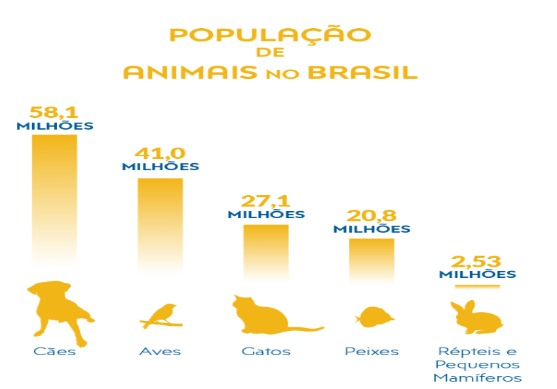
\includegraphics{exemplos/diagramas/População_Animais.jpeg}
    \caption{A população de animais no Brasil no ano de 2021.}
    \label{fig:População_Animais}
    \fonte{Instituto Pet Brasil apud IBGE}
\end{figure}
\\
Considerando o grande número de pessoas com Pets(LINK AQUI) e o carinho que possuem por eles, criou-se   um certo medo de como seus animais serão tratados. Segundo o (Graf , 2016)(LINK AQUI) os donos de animais de estimação, no momento de escolher profissionais para cuidar de seus Pets(LINK AQUI), possuem muitos receios, no que tange a qualidade do serviço e o cuidado do profissional, além disso, o preço do serviço (Gráfico 2)(LINK AQUI).
Um método muito efetivo de conhecer a qualidade de um serviço é por indicação que uma pessoa recebe de um amigo ou conhecido,  nesse âmbito, a aplicação busca disponibilizar avaliações dos parceiros feitas por outros usuários. 
\begin{figure}
    \centering
    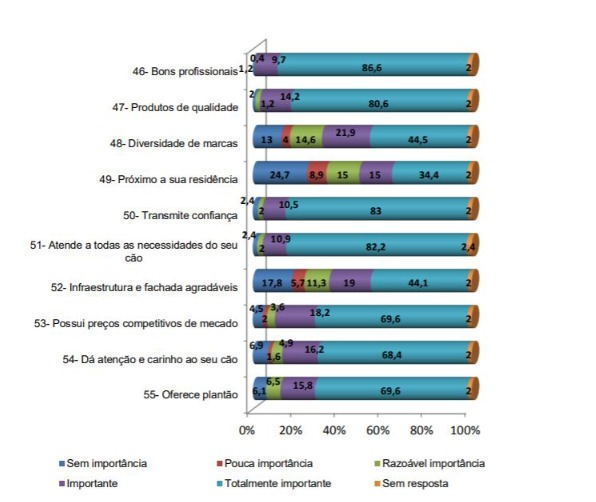
\includegraphics{exemplos/diagramas/graf_analise.jpeg}
    \caption{Principais motivos de escolha de Pet Shops. Os números indicam o número das perguntas, no questionário original da referência Graf (2016)(LINK AQUI)}
    \label{fig:graf_analise}
    \fonte{Graf (2016)(LINK AQUI)}
\end{figure}
\\

\subsection{Análise de concorrência}
Uma das ferramentas importantes no design de projetos é analisar empreendimentos similares e verificar os pontos positivos e negativos para justificar a criação de uma nova proposta. Entre os concorrentes atuais temos:
\begin{itemize}
    \item \textbf{PetDrive:}
        \begin{enumerate}
            \item \textbf{Pontos positivos:}
            Um dos aplicativos mais conhecidos pelo transporte de animais de estimação com seus donos, tendo como um de seus diferenciais o agendamento e equipamentos de transporte de animais dentro do carro disponibilizado pela empresa.
            \item \textbf{Pontos negativos:}
            Não disponibiliza a opção do cliente usar o seu próprio equipamento e não há a opção de viagens de animais desacompanhados.
    \end{enumerate}
    \item \textbf{Uber Pets}:
    \begin{enumerate}
            \item \textbf{Pontos positivos:}
            Conhecido dentro e fora do Brasil, interface intuitiva.
            \item \textbf{Pontos negativos:}
            Os carros não são adaptados para transporte de animais, não transportam o pet sozinho.
    \end{enumerate}
    \item \textbf{Mr. taxidog:}
    \begin{enumerate}
            \item \textbf{Pontos positivos:}
            Empresa antiga  no mercado, com profissionais qualificados e preparados no transporte de cachorros.
            \item \textbf{Pontos negativos:}
            Não é possível transportar outros pets como gatos e pássaros. Funciona somente no estado do Paraná.
    \end{enumerate}
    \item \textbf{Driver dog:}
    \begin{enumerate}
            \item \textbf{Pontos positivos:}
            Empresa com mais de 14 anos no mercado. Possui profissionais qualificados para lidar com cães, e transporte por longas distâncias.
            \item \textbf{Pontos negativos:}
            Não é possível transportar outros seres como gatos, coelhos,etc.
    \end{enumerate}
    \item \textbf{Dog hero:}
    \begin{enumerate}
            \item \textbf{Pontos positivos:}
            Possui profissionais qualificados na área de saúde animal, hospedagem de pets e creche. Está disponível em todo o Brasil.
            \item \textbf{Pontos negativos:}
            Aplicativo pouco intuitivo de transporte com veículo.
    \end{enumerate}
\end{itemize}

Analisando todos os concorrentes vemos que existe espaço para competitividade e crescimento de um novo produto. Portanto, o Carrara Pets busca trazer uma nova experiência para seus clientes , trazendo inovação, facilidade e mais funcionalidades para o cliente e seu pet, não se propondo a só transportar e cuidar dos pets, mas também buscar parcerias que agreguem mais valor para o negócio e satisfação ao consumidor final.

\begin{quadro}[thb]
\centering
\ABNTEXfontereduzida
\caption{Comparativo entre concorrentes}
\label{quadro-poluido-limpo-desalinhado}
\begin{tabular}{|l|l|l|l|l|l|l|}
\hline
\thead{Recursos} & \thead{Pet\\Driver} & \thead{Uber\\Pets} & \thead{Carrara\\Pets} & \thead{Mr.\\Taxidog} & \thead{Driver\\Dog} & \thead{Dog\\Hero}  \\
\hline
Transportar animais & \circlemark & \circlemark & \circlemark & \circlemark & \circlemark & \\
\hline
Corridas agendadas &\circlemark& &\circlemark& & &\circlemark\\
\hline
Serviços prestados pelo motorista & & &\circlemark& & &\\
\hline
Acompanhamento de viagem  &\circlemark&\circlemark&\circlemark& & &\circlemark\\
\hline
Hospedagem & & &\circlemark& & &\circlemark\\
\hline
Creche & & &\circlemark& & &\circlemark\\
\hline
Viagem compartilhada & & & &\circlemark& & \\
\hline
\end{tabular}
\fonte{Os autores.}
\end{quadro}

\section{Estrutura do Documento}
O presente documento está estruturado em 5 capítulos. O Capítulo 1(LINK AQUI), traz a contextualização do tema do projeto e a solução proposta, além de mostrar o objetivo geral e o objetivo específico, que deseja-se conquistar no desenvolvimento da aplicação. Ademais, possui a justificativa para a solução e uma análise de concorrência, demonstrando quais seriam os recursos disponíveis na plataforma Carrara Pets. Para finalizar, o capítulo contém esta seção para explicar a estrutura do documento. \\
No Capítulo 2(LINK AQUI), Revisão da Literatura, reúne-se as referências que forneceram embasamento para o trabalho. Neste capítulo, o leitor contará com temas referentes à aplicativo e público alvo, pontos principais da aplicação.\\
O Capítulo 3(LINK AQUI), Gerenciamento do Projeto, possui seções direcionadas a organização da equipe, falando sobre a metodologia que está sendo utilizada, links que contém algumas informações, como o canal do YouTube, blog da equipe e entre outros. \\
O Capítulo 4(LINK AQUI), Desenvolvimento do Projeto, aborda sobre as tecnologias utilizadas, viabilidade da aplicação, mostra os itens do escopo do projeto, apresenta a arquitetura da aplicação, a modelagem de dados e o diagrama de classes; explica sobre os padrões de projeto, sobre a segurança da informação e outros tópicos referentes ao desenvolvimento da aplicação.\\
Por fim, o Capítulo 5(LINK AQUI) é composto pelo resumo do projeto, explicitando as dificuldades de implementar o Carrara Pets e os obstáculos que apareceram durante o desenvolvimento e as funcionalidades futuras que poderão ser adicionadas à aplicação.\\
Além destes capítulos, o documento contém uma seção de Apêndice, com os documentos extras criados pela equipe ao decorrer do desenvolvimento, que acrescentam informações e melhoram o entendimento do projeto.


\newpage
\section{Processos}
\begin{itemize}
    \item Acompanhamento do veículo 
    \item Diagnóstico do atendimento (Veterinário)
    \item Possível cobrança em casos de compra de remédio
    \item Definição de rota para viagem
    \item Método de fidelidade (Pontos)
    \item Salvar acontecimentos da corrida em forma do tempo
    \item Fidelidade de motorista “X” pet (rotina)
    \item Compatibilidade do porte do pet com dimensões do veículo
    \item Validação do cadastro do motorista (Nome, Idade, Carro, Placa, CNH, CPF, Pré-entrevista com psicólogo(a))
    \item Cadastro de características
    \item Cadastro do pet (Tamanho, Peso, Porte, Temperamento)
    \item Cadastro do dono (Nome, CPF, Idade, Telefone, Endereço...)

\end{itemize}



% ---
% Capitulo de revisão de literatura
% ---
\chapter{Revisão da Literatura}

Na antiguidade, os seres humanos e outros animais caçavam devido a seu instinto, porém em algum momento, os seres humanos entenderão que ao domesticar esses animais poderiam ter maior efetividade no seu dia a dia. No decorrer do tempo, o ser humano descobriu que ao coexistir com animais, eles os tornavam mais fortes e felizes, foram inseridos cada vez mais em seu cotidiano até se tornarem parte da família, como seres de estimação, companheiro fiel e um apoio emocional (PESSANHA; PORTILHO, 2008)(LINK AQUI).
Olhando a sociedade moderna, onde esses animais se tornaram extremamente valorizados, de modo que chegam a substituir filhos. Muitas pessoas desistem de ter filhos para ter um animal tratado como tal (PESSANHA; PORTILHO, 2008)(LINK AQUI).

\section{Aplicativos}
Com o desenvolvimento da tecnologia o uso de aparelhos celulares e seus aplicativos têm se tornado essenciais no cotidiano das pessoas, por inúmeros motivos como facilidade para acessar contas bancárias, solicitar transporte, pedir uma refeição etc. Tudo isso de maneira rápida e extremamente acessível. Segundo pesquisas, o Brasil possui um grande potencial no âmbito de dispositivos móveis, cerca de 29\% da população utiliza aplicativos para atividades corriqueiras. Outra pesquisa mostra que as pessoas do Brasil ficam em torno de 3 horas em frente ao celular diariamente, superando países como EUA. (CARVALHO, 2003; GLOBOESPORTE.COM, 2019; SANTOS, 2020; BRITO, 2021)(LINK AQUI).\\
No projeto, a ideia de criar um aplicativo ao invés de um WebApp ou uma aplicação Web, deu-se o intuito de ter maior credibilidade e funcionalidade na aplicação, além de usar uma baixa quantidade de dados móveis para o cliente final.

\section{Público alvo}
Silva (2021) apud Graf (2016) Diz que os animais são atualmente tratados como membros da família. Segundo Silva et.al. (2021), a relação entre seres domesticados e seus donos pode ser separada em:
\begin{itemize}
    \item \underline{" Afeto: O dono usa mais serviços/produtos de alta qualidade, como enfeites, xampu\\, roupas etc.;" }
    \item \underline{"Interação: Onde o dono contrata serviços de adestramento para adequar o animal \\ao seu estilo de vida e produtos para o bem-estar dele;"}
    \item \underline{"Substituição humana: O consumidor substitui as relações humanas, como filhos ou \\amigos, pelo animal de estimação, pagando por atividades de tratamentos \\veterinários de luxo, adestramento e atividades geralmente associadas a relações humanas,\\ como funerais.”}
\end{itemize}

% ---

% ---

% ---


% Para facilitar a manutenção é sempre melhore criar um arquivo por capitulo, para exemplo isso não é necessário 
% Para facilitar a manutenção é sempre melhore criar um arquivo por capitulo, para exemplo isso não é necessário 

%---------------------------------------------------------------------------------------
\chapter{Modelo Teórico e Pressupostos (ou Hipóteses) da Pesquisa}




%---------------------------------------------------------------------------------------
\chapter{Métodos de Pesquisa}
\explicacao{Para trabalho da Pós Graduação}


\section{Tipo de Pesquisa}


\section{Plano Amostral (se Pesquisa Quantitativa)}


\section{Instrumento de Pesquisa e Escalas Utilizadas (Escalas se Pesquisa Quantitativa)}


\section{Coleta de Dados}


\section{Análise de Dados}



%---------------------------------------------------------------------------------------
\chapter{Resultados da Pesquisa}
\explicacao{Para trabalho da Pós Graduação}

\section{Discussão dos Resultados Observados}


%---------------------------------------------------------------------------------------





% exemplos de escrita LaTeX
\chapter{Exemplos \LaTeX}
\label{cap-exemplos}

\explicacao{ATENÇÃO : Este capítulo e os seguintes demonstram como fazer no {\LaTeX} portanto devem ser lidos em conjunto com o código fonte desse documento}

% exemplo de como inserir uma referencia adicional no sumario (normalmente não utilizado em um trabalho acadêmico)
\addcontentsline{toc}{chapter}{Exemplos que devem ser lidos (mas esse tipo de indicação não vai em um trabalho acadêmico) :-)}

Esse capítulo tem exemplos de escrita utilizando o {\LaTeX}  utilizando \abnTeX, é muito simples escrever em \textbf{negrito}, \textit{itálico} \footnote{apesar de que nesse documento \mostraComandoLaTeX{textit} \mostraComandoLaTeX{emph} tem comportamento parecido é recomendável utilizar \mostraComandoLaTeX{textit} de forma genérica para itálico}, ....


Existem diversos tutoriais para uso de \LaTeX, se você está utilizando esse modelo não precisará se preocupar com muitos dos detalhes técnicos do \LaTeX \space e cuidar somente do seu texto.

Escolha seu editor : \url{https://en.wikipedia.org/wiki/Comparison\_of\_TeX\_editors}, apesar do overleaf sem bem prático, nem todas as funções estão disponíveis na versão gratuita e você pode instalar gratuitamente em seu computador um compilador \LaTeX \space e utilizar um sistema de controle de versão para gerenciar seu documento.


\section{Normas ABNT}

Esse documento modelo já resolve boa parte da padronização NBR 14.724:2011 \cite{NBR14724:2011} que deve ser seguida e inclusive alguns pontos que não são claros pelo modelo de padronização do \ac{ifsp}.

Leia os documentos do {\abnTeX} e do \ac{ifsp}:
\begin{itemize}
    \item \url{https://www.abntex.net.br/}
    
    \item \acs{faq} : \url{https://github.com/abntex/abntex2/wiki/FAQ}
    
    \item \url{http://mirror.unl.edu/ctan/macros/latex/contrib/abntex2/doc/abntex2.pdf}
    
    \item \waUrl{https://spo.ifsp.edu.br/biblioteca?id=184}
\end{itemize}

No \ac{ifsp} você pode acessar todas as normas \ac{abnt} sem custo, as informações estão disponíveis no endereço \waUrl{https://www.ifsp.edu.br/index.php/outras-noticias/52-reitoria/2329-alunos-e-servidores-do-ifsp-podem-acessar-abnt-via-web.html}.

Apesar de alguns elementos serem opcionais na \ac{abnt} eles foram definidos como obrigatórios (folha de rosto, resumo, lista de siglas, lista de ilustrações, glossário etc), nos trabalhos completos de projetos de informática do \ac{ifsp} campus São Paulo. Documentos menores como propostas de projeto, documento de \ac{poc} não necessitam desses elementos, mas alguns podem ser uteis para ajudar no estudo do {\LaTeX} em preparação para o documento final.

\begin{itemize}
    \item Logotipo da instituição, não é citado na \ac{abnt} nem no manual de normalização do \ac{ifsp}, mas aparece em uma imagem do documento de normalização, foi definido que não deve ser incluído na capa;
    
    \item Nome da instituição que é opcional na capa, deve ser utilizado;
    
\end{itemize}



\section{Detalhes textuais}

O documento é dividido em capítulos, e cada capítulo dividido em seções utilizando o \abnTeX \space você pode dividir seus documentos nos níveis de acordo com os comandos:

\begin{itemize}
    \item \mostraComandoLaTeX{chapter}  (1);
    
    \item \mostraComandoLaTeX{section} (1.1);
    
    \item \mostraComandoLaTeX{subsection} (1.1.1);
    
    \item \mostraComandoLaTeX{subsubsection} (1.1.1.1);
    
    \item \mostraComandoLaTeX{subsubsubsection} (1.1.1.1.1).
    
\end{itemize}

Tenha em mente que normalmente se utiliza no máximo o nível \mostraComandoLaTeX{subsection}.
Ao definir as divisões do seu trabalho utilizando as diretivas do \LaTeX, elas são automaticamente inseridas no sumário do documento.


\subsection{Caracteres Reservados e auxiliares}



Alguns caracteres são reservados no \LaTeX \space e por isso para utilizar esses caracteres é necessário utilizar uma forma diferenciada de escrita. É possível utilizar a macro \mostraComandoLaTeX{symbol} com o código \ac{ascii} do caracter desejado, veja no código fonte desse texto como utilizar corretamente esses itens.


\begin{itemize}
\item barra invertida : \textbackslash   \symbol{92}    $\backslash$;
\item til  :  \symbol{126} ;
\item cifrão : \$;
\item sublinhado, \textit{underscore}, \textit{underline} : \_;
\item \enquote{aspas} as macros \mostraComandoLaTeX{enquote} / \mostraComandoLaTeX{textquote} garantem o espaçamento correto, se utilizar diretamente as ASPAS o espaçamento é perdido;
% https://tex.stackexchange.com/questions/80395/no-space-after-closing-double-quote
\item marcadores : \cmark\ \xmark\ \circlemark\ \ding{100} \ - ver mais no \refanexo{pifont-quickref};
\item chaves : \} \{.
\end{itemize}

\subsection{Listas}

Em uma lista de itens cada item deve ser terminado por ponto e virgula, exceto o ultimo item que deve ter um ponto final.

\begin{itemize}
\item item 1;
\item item 2;
\item item ..;
\item item final.
\end{itemize}


\chapter{Referências}
ABINPET. Mercado Pet Brasil 2021. Disponível em: <http://www.abinpet.org.br/download/abinpet_folder_2021.pdf> Acesso em 14 de Abril de 2022.
INSTITUTO PET BRASIL.Censo Pet: 139,3 milhões de animais de estimação no Brasil.2019.Disponível em: <http://institutopetbrasil.com/imprensa/censo-pet-1393-milhoes-de-animais-de-estimacao-no-brasil/> Acesso em: 14 de Abril de 2022.
GOVERNO FEDERAL DO BRASIL. O Brasil registrou mais de 234 milhões de acessos móveis em 2020. Agência Nacional de Telecomunicações. 2021. Disponível em: <https://www.gov.br/pt-br/noticias/transito-e-transportes/2021/05/brasil-registrou-mais-de-234-milhoes-de-acessos-moveis-em-2020> Acesso em: 14 de Abril de 2022.
HEROKU. Heroku Pricing. 2020. Disponível em: <https://www.heroku.com/pricing#app-types-header>.Acesso em: 14 abr. 2022.
RIBEIRO, A. F. de A. Cães Domesticados e os benefícios da interação. Revista Brasileira de Direito Animal, Salvador, v. 6, n. 8, 2014. DOI: 10.9771/rbda.v6i8.11062. Disponível em: https://periodicos.ufba.br/index.php/RBDA/article/view/11062. Acesso em: 14 abr. 2022.
SILVA, N. A.; MARISCO, G. A RELAÇÃO DE ANIMAIS DOMÉSTICOS NA EDUCAÇÃO E SAÚDE. Interfaces Científicas - Saúde e Ambiente, [S. l.], v. 7, n. 1, p. 71–78, 2018. DOI: 10.17564/2316-3798.2018v7n1p71-78. Disponível em: https://periodicos.set.edu.br/saude/article/view/5491. Acesso em: 14 abr. 2022.
SOUZA, A. S. de. Direitos dos animais domésticos: análise comparativa dos estatutos de proteção. Revista de Direito Econômico e Socioambiental. v. 5, n. 1, p. 110–132, 2014. Disponível em: <https://periodicos.pucpr.br/direitoeconomico/article/view/6242>. Acesso em: 14 abr. 2022.
GOOGLE PLAY CONSOLE. Disponível em: <https://play.google.com/console/u/0/signup>.Acesso em: 16 abr. 2022.
APPLE DEVELOPER PROGRAM.Isenção da taxa de assinatura no Apple Developer Program
. Disponível em: <https://play.google.com/console/u/0/signup>.Acesso em: 16 abr. 2022.
Docker. Docker Pricing. 2022. Disponível em: <https://www.docker.com/pricing/>.Acesso em: 16 abr. 2022.
GREGOL, R. E. W. Recursos de escalabilidade e alta disponibilidade para aplicações web.Repositório de Outras Coleções Abertas, p. 17–18, 2011.
ENDEAVOR. Quão longe sua ideia pode ir? Descubra avaliando a escalabilidade dela. 2015. Disponível em: <https://endeavor.org.br/estrategia-e-gestao/escalabilidade/>.Acesso em: 17 abr. 2022.
GOOGLE DEVELOPERS. Disponível em: <https://developer.android.com/docs/quality-guidelines/core-app-quality?hl=pt-br#sc>.Acesso em: 18 abr. 2022.
BRASIL. Lei Geral de Proteção de Dados (2018). 2018. Disponível em: <http://web.archive.org/web/20200915225322/http://www.planalto.gov.br/ccivil_03/_ato2015-2018/2018/lei/L13709.htm>. Acesso em: 18 abr. 2022.
 MARTIN FOWLER.Continuous Integration. 2001.Disponível em: <https://martinfowler.com/articles/continuousIntegration.html>.Acesso em: 18 abr. 2022.
PESSANHA, L.; PORTILHO, F. Comportamentos e padrões de consumo familiar em torno dos “pets”. IV ENEC - Encontro Nacional de Estudos do Consumo, 2008.
GRAF, C. T. O comportamento do consumidor no mercado pet e a relação entre os cães e as pessoas. Universidade Regional do Noroeste do Estado do Rio Grande do Sul, 2016.
CHEN, A.; HUNG, K.; PENG, N. A cluster analysis examination of pet owners ’consumption values and behavior –segmenting owners strategically. Journal of Targeting, Measurement and Analysis for Marketing, v. 20, n. 2, p. 117–132, 2012.
Silvaet.al.Petshow.2021.Disponível em:<https://svn.spo.ifsp.edu.br/svn/a6pgp/S202001-PI/HYVE/Documentos/5-EntregaFina>.Acesso em: 01 mai. 2022.
PRODEST.O uso de aplicativos na sociedade.Disponível em:
<https://prodest.es.gov.br/o-uso-de-aplicativos-na-sociedade#:~:text=Os\%20aplicativos\%20fazem\%20cada\%20vez,op\%C3\%A7\%C3\%B5es\%20de\%20lazer\%20com\%20facilidade.> Acesso em: 03 mai. 2022.
CARVALHO, J. O. F. D. O papel da interação humano-computador na inclusão digital. Transformação, V. 15, n. spe, p. 75-89. Campinas, Dezembro, 2003 .Disponível em: <http://www.scielo.br/scielo.php?script=sci_arttext&pid=S0103-37862003000500004&lng=en&nrm=iso>. Acesso em: 03 mai. 2022.
GLOBOESPORTE.COM. Uso de aplicativos de saúde deve aumentar nos
próximos anos, segundo pesquisa. Grupo Globo. Rio de Janeiro.2019. Disponível
em:<https://globoesporte.globo.com/eu-atleta/noticia/uso-de-aplicativos-de-saude-deve-aumentar-nos-proximos-anos-segundo-pesquisa.ghtml> .  Acesso em: 03 mai. 2022
BRITO, S. Quem usa mais o smartphone: Brasil ou Estados Unidos? Revista Veja digital. Editora Abril. Janeiro de 2021. Disponível em: 
<https://veja.abril.com.br/tecnologia/quem-usa-mais-o-smartphone-brasil-ou-estados-unidos/> . Acesso em: 03 mai. 2022.
SANTOS, A. Brasil, segundo país onde o mercado de aplicativos mais cresce.Terra.2020. Disponível em:<https://www.terra.com.br/noticias/dino/brasil-segundo-pais-onde-o-mercado-de-aplicativos-mais-cresce,1fd9d38aa995ad8ca1243f6c58080f79u2ee8tfj.html#:~:text=Os\%\%20realizados\%20pela\%20empresa,m\%C3\%A9dio\%20real\%20de\%2030\%20apps.&text=Houve\%20um\%20aumento\%20de\%2030,aplicativos\%20do\%20Google\%2C\%20em\%202020> .  Acesso em: 03 mai. 2022.
INSTITUTO PET BRASIL. Censo Pet: 139,3 milhões de animais de estimação no Brasil. 2019. Disponível em: <http://institutopetbrasil.com/imprensa/censo-pet-1393-milhoes-de-animais-de-estimacao-no-brasil/>. Acesso em: 19 mai. 2022.
PUGA, E. F. e. M. G. S. Banco de dados: Implementação em SQL, PL/SQL e Oracle 11g. 1. ed. São Paulo: Pearson Universidades, 2013. Acesso em: 21 mai. 2022.
IBM. Arquitetura de três camadas. 2020. Disponível em: 
<https://www.ibm.com/br-pt/cloud/learn/three-tier-architecture#toc-benefcios--jxGrdA7u>. Acesso em: 22 mai. 2022.
https://www.w3schools.com/js/js_conventions.asp




\subsection{Elementos não textuais / Ilustrações}
\label{elementos-nao-textuais}

Elementos não textuais são aqueles que auxiliam o entendimento, não podem ficar \enquote{jogados} no texto, devem ser citados, cada elemento deve ser identificado por um \mostraComandoLaTeX{label} único que permite a sua referencia, no texto utilizando \mostraComandoLaTeX{ref} ou \mostraComandoLaTeX{autoref}, esses elementos quando definidos corretamente também são inseridos nas listas presentes antes do sumário.

Cuidado com o artigo \textbf{O/A} antes da Figura, Tabela ou Quadro referenciado, deve ser compatível com o tipo da ilustração.

Lembre que o \LaTeX \  vai posicionar os elementos  da melhor maneira possível dentro do documento, sempre faça as referencias utilizando os comandos específicos, nunca utiliza \enquote{acima}, \enquote{"baixo}, \enquote{a seguir}, etc... 

O posicionamento desses elementos é feito pelas rotinas do pacote float, leia a documentação em  \url{http://linorg.usp.br/CTAN/macros/latex/contrib/float/float.pdf}. É recomendável utilizar as opções de posicionamento \textbf{htb}, a opção \textbf{H} deverá ser utilizada somente como ultima alternativa de posicionamento e em alguns casos a utilização de \mostraComandoLaTeX{FloatBarrier} pode também melhorar o resultado se utilizada com cuidado.

Lembre que se houver uma grande distancia entre a ilustração no documento \ac{pdf} e sua definição original no documento isso significa que existe muito pouco texto em seu documento e isso não oferece muitas opções para o {\LaTeX} organizar as ilustrações. Você precisa nesse caso melhorar a descrição textual das ilustrações.


Para casos onde existe uma grande distancia entre a ilustração e o ponto de referencia no texto esse modelo possui macros \mostraComandoLaTeX{autorefwithpage} e \mostraComandoLaTeX{autorefwithpagedistance} a primeira sempre indica página onde a ilustração foi colocada e a segunda somente se a ilustração estiver mais distante que o número de páginas indicado como parâmetro, Ex. \autorefwithpage{fig_logo_A3}. Isso deve ser utilizado somente quando existe mais de uma referencia para mesma ilustração e não para deixar a ilustração distante de uma única referencia.

O titulo da ilustração deve ser apresentado sempre no topo (conforme \citetitle{NBR14724:2011}, era na parte inferior na  \citetitle{NBR14724:2005}), e a fonte deve ficar na parte inferior \cite{NBR14724:2011}. A norma não possui um exemplo direto do uso das fontes e é possível encontrar exemplos com e sem ponto final nas fontes das ilustrações. Considerando a utilização de ponto no manual do \ac{ibge} nesse modelo foi escolhido utilizar o ponto final na fonte das ilustrações.





% ---
\subsection{QR-Code}
% ---
\index{qr-code}
\explicacao{Entendam que faz sentido colocar aqui nesse MODELO uma seção chamada QR-Code pois está sendo explicada a forma de utilização, mas em um documento normal onde o QR-Code é utilizado para apresentar uma URL não faz sentido, já que ele é somente uma ferramenta como um gráfico de pizza}


A utilização de códigos \ac{qr} facilita o acesso de endereços da internet a partir de dispositivos móveis com câmera.
As Figuras \ref{qr-url-1} e \ref{qr-url-2} demonstram dois exemplos de endereços apresentados com essa tecnologia.


Para facilitar a utilização dos códigos \ac{qr}, deve-se tomar cuidado para não deixa-los alinhados na vertical se houverem vários seguidos, pois dificulta a seleção a partir da câmera no dispositivo móvel.

Os endereços também devem ter seu \ac{url} apresentada de forma que mesmo um usuário que esteja fazendo a leitura do documento eletrônico também vai conseguir acessar o endereço indicado. Observe que as figuras de demonstração possuem tanto o código \ac{qr} como o \ac{url}.

Um exemplo para utilização de mais códigos de barra pode ser visto em : \urlmodelo.

Atenção, alguns compiladores podem ter problemas em utilizar a biblioteca \textbf{pstricks} necessária para gerar QR-Codes, no sharelatex em 2017-05 a compilação ocorre perfeitamente utilizando a opção de compilador "XeLatex", ele é mais lento que outras opções.


\begin{figure}[htb]
\caption{\label{qr-url-1}URL para acesso ao documento exemplo}
\begin{pspicture}(25mm,25mm)
\psbarcode{\urlmodelosimples}{eclevel=H width=1.0 height=1.0}{qrcode}
\end{pspicture}
\legend{\urlmodelo}
\fonte{Os Autores.}
\end{figure}


\explicacao{o repositório indicado pela \autoref{qr-url-2} não está sendo atualizado, utilize a versão disponível no overleaf}

% colocando figura qrcode na direita para facilitar o uso da camera deixando cada qrcode em um alinhamento diferente
% se deixar os dois qrcodes um em cima do outro dificulta acessar o desejado
\begin{figure}[htb]
\caption{\label{qr-url-2}Repositório original de classes IFSP \LaTeX}
\begin{flushright}
\begin{pspicture}(25mm,25mm)
\psbarcode{https://github.com/ivanfmartinez/latexlib/tree/master/ifsp}{eclevel=H width=1.0 height=1.0}{qrcode}
\end{pspicture}
\legend{\url{https://github.com/ivanfmartinez/latexlib/tree/master/ifsp}}
\fonte{Os Autores.}
\end{flushright}

\end{figure}


\subsection{Organizando pendências}

Durante o desenvolvimento de um trabalho escrito é normal que alguns elementos sejam gerados posteriormente, mas é importante se organizar para não esquecer de fazer os ajustes necessários. Para isso recomendo a utilização do pacote \textbf{todonotes} que oferece diversos recursos para gerar lembretes das pendencias. O manual do \textbf{todonotes} está disponível no \autoref{manual-todonotes}\footnote{observe que existe um erro nesse documento, já que a referencia deveria ser Anexo e aparece como Apêndice,  existe um \textit{bug} no abntex2 ao referenciar anexos, para fazer corretamente veja \url{https://github.com/abntex/abntex2/issues/76} e utilize \mostraComandoLaTeX{refanexo} que está disponível nesse modelo.}.

É possível fazer anotações de pendencias inclusive indicando as pessoas responsáveis por elas, % nao mover o todo pois foi feito no meio do paragrafo exatamente para demonstrar um possível problema de formato
\todo[inline,author=Pessoa1]{fazer revisão das imagens do texto} e para facilitar a visualização criar imagens que funcionam como marcadores para figuras que serão incluídas posteriormente.

Cuidado ao utilizar as anotações \textit{inline} pois o texto ficara quebrado, como no paragrafo anterior.


\begin{figure}[htb]
    \centering
	\caption{\label{fig_todo1}Imagem que ainda não foi gerada}
	\missingfigure[figwidth=10cm]{você está atrasado pois ainda não criou esta figura}
	\fonte{dados do Projeto.}
\end{figure}



\subsection{Tabelas e Quadros}
\label{tabelas-e-quadros}
Quadros e Tabelas são informações tabulares, mas Tabelas tem como objetivo apresentar números. A ‘norma’ 14724 \cite[3.32]{NBR14724:2011} define a Tabela como sendo uma \enquote{forma não discursiva de apresentar informações das quais o dado numérico se destaca como informação central} e que devem seguir padronização do \ac{ibge}  \cite[5.9]{NBR14724:2011}. O \ac{ibge} padronizou a apresentações de dados tabulares em 1993 \cite{tabular-ibge}.

Informações adicionais sobre o de tabelas no {\LaTeX} podem ser obtidas em  \url{https://en.wikibooks.org/wiki/LaTeX/Tables}.

Antes de utilizar \index{longtable}\textbf{longtable} procure reorganizar o seu layout ou quebrar manualmente em múltiplos quadros / tabelas, pois isso ainda facilita a compreensão pelo leitor.

% https://biblioteca.ibge.gov.br/visualizacao/livros/liv23907.pdf

\index{quadros}O \autoref{quadro-exemplo} é um exemplo de dados tabulares gerados em 
\LaTeX.



\begin{quadro}[htb]
\centering
\ABNTEXfontereduzida
\caption[Níveis de investigação]{Níveis de investigação}
\label{quadro-exemplo}
\begin{tabular}{|p{2.6cm}|p{6.0cm}|p{2.25cm}|p{3.40cm}|}
  \hline
   \thead{Nível de\\Investigação} & \thead{Insumos}  & \thead{Sistemas de\\ Investigação}  & \thead{Produtos}  \\
    \hline
    Meta-nível & Filosofia\index{filosofia} da Ciência  & Epistemologia &
    Paradigma  \\
    \hline
    Nível do objeto & Paradigmas do metanível e evidências do nível inferior &
    Ciência  & Teorias e modelos \\
    \hline
    Nível inferior & Modelos e métodos do nível do objeto e problemas do nível inferior & Prática & Solução de problemas  \\
   \hline
\end{tabular}
\fonte{O Autor.}
\end{quadro}



\index{tabelas}Já a \autoref{tab-exemplo} foi criada conforme o padrão \citeonline{tabular-ibge} requerido pelas normas da \ac{abnt} para documentos técnicos e acadêmicos. Observe que não existem bordas laterais e nem linhas separadoras em uma Tabela e as colunas numéricas tem alinhamento à direita. 

\begin{table}[htb]
\centering
\caption{Métricas de desenvolvimento}
\label{tab-exemplo}
\begin{tabular}{p{2.6cm}rrr}
    \hline
   \thead{Item} & \thead{Janeiro}  & \thead{Fevereiro}  & \thead{Março}  \\
    \hline
    Classes & 2  & 10 & 20  \\
    Linhas & 100  & 250 & 543 \\
    \hline
\end{tabular}
\fonte{Os autores.}
\end{table}

\def\equationautorefname~#1\null{%
  Equação~(#1)\null
}


Para facilitar a criação de tabelas e quadros existem algumas ferramentas como o Tables Generator \url{http://www.tablesgenerator.com/latex_tables} que permite a criação de forma visual gerando o código \LaTeX\ correspondente. E o site \url{https://www.latex-tables.com/} permite converter planilhas em código \LaTeX.


\index{equação}\index{Pitágoras}A \autoref{eq-pythagoras} demonstra que também é possível escrever equações diretamente em \LaTeX

\begin{equation}\label{eq-pythagoras}
a^2+b^2=c^2\,.
\end{equation}






% ---
\subsection{Figuras}
\label{sec_figuras}
% ---

\index{figuras}Figuras podem ser criadas diretamente em \LaTeX,
como o exemplo da \autoref{fig_circulo}, ou inseridas a partir de arquivos externos como a \autoref{fig_logo}, que é o Logotipo do \ac{ifsp}. \index{logotipo}

% Aqui foi utilizada uma figura unica para demostrar a diferença de qualidade entr e vetorizado e não vetorizado pois fica mais simples, já que cada leitor pode ver esse documento em monitores com diferentes qualidades...
As figuras externas devem possuir boa qualidade e preferencialmente serem vetorizadas para se obter o melhor resultado. A \autoref{fig:nao_vetorizado_e_vetorizado} apresenta duas versões de uma mesma imagem demonstrando a variação de qualidade que pode acontecer quando não for utilizada a versão vetorizada, quando a figura possui elementos textuais pode até inviabilizar a leitura. As Figuras \ref{fig:uml_dia_nao_vetorizado_jpeg}, \ref{fig:uml_dia_vetorizado_eps} e \ref{fig:uml_dia_vetorizado_svg} foram reduzidas propositalmente no documento para demonstrar a diferença entre os formatos de arquivo. A diferença fica mais perceptível quando o documento é impresso ou quando existem textos pequenos e é necessário fazer zoom para visualização.

Procure criar suas imagens e diagramas pensando em utilizar impressão em preto-e-branco ou escala de cinza. Isto é importante, principalmente quando se pretende publicar o trabalho, uma vez que a maioria das publicações são somente em preto-e-branco. Outro benefício é o custo de impressão, normalmente menor para páginas preto-e-branco em relação a páginas coloridas.

Para diagramas em \ac{uml} o PlantUML pode ser utilizado para gerar código {\LaTeX} como exemplo na  \autoref{diagramauml}.


Se não houver a possibilidade de utilização de uma imagem vetorizada e existem diversos detalhes utilize \ac{png} em vez de \gls{jpg} ou outros formatos de menor qualidade, observe as diferenças nos exemplos apresentados em :  \waUrlTitle{https://tex.stackexchange.com/questions/136087/selecting-best-file-extension-for-graphics-figures-pictures}{Selecting best file extension for graphics figures pictures}.


\begin{figure}[htb]
	\caption{\label{fig_circulo}A delimitação do espaço}
	\begin{center}
	    \setlength{\unitlength}{5cm}
		\begin{picture}(1,1)
		\put(0,0){\line(0,1){1}}
		\put(0,0){\line(1,0){1}}
		\put(0,0){\line(1,1){1}}
		\put(0,0){\line(1,2){.5}}
		\put(0,0){\line(1,3){.3333}}
		\put(0,0){\line(1,4){.25}}
		\put(0,0){\line(1,5){.2}}
		\put(0,0){\line(1,6){.1667}}
		\put(0,0){\line(2,1){1}}
		\put(0,0){\line(2,3){.6667}}
		\put(0,0){\line(2,5){.4}}
		\put(0,0){\line(3,1){1}}
		\put(0,0){\line(3,2){1}}
		\put(0,0){\line(3,4){.75}}
		\put(0,0){\line(3,5){.6}}
		\put(0,0){\line(4,1){1}}
		\put(0,0){\line(4,3){1}}
		\put(0,0){\line(4,5){.8}}
		\put(0,0){\line(5,1){1}}
		\put(0,0){\line(5,2){1}}
		\put(0,0){\line(5,3){1}}
		\put(0,0){\line(5,4){1}}
		\put(0,0){\line(5,6){.8333}}
		\put(0,0){\line(6,1){1}}
		\put(0,0){\line(6,5){1}}
		\end{picture}
	\end{center}
	\fonte{Modelo Canônico ABNTeX2.}
\end{figure}


\begin{figure}[htb]
    \centering
	\caption{\label{fig_logo}Logotipo \ac{ifsp}}
	
\includegraphics{\ifspprefixo/logo-02.jpg}
	\fonte{\ac{ifsp}.}
\end{figure}

\begin{figure}
    \centering
    \caption{Exemplo de imagem não vetorizada e vetorizada}
    \label{fig:nao_vetorizado_e_vetorizado}
	
\includegraphics[width=0.95\textwidth]{erros/exemploVetorizacao.png}
    \fonte{\citeonline{vetorizacao}.}
\end{figure}
    

% Essas imagens foram reduzidas na apresentação para demonstrar o efeito da alteração de escala em imagens não vetorizadas
\begin{figure}
    \centering
    \caption{Exemplo de diagrama - salvo em imagem não vetorizada - JPEG}
    \label{fig:uml_dia_nao_vetorizado_jpeg}
	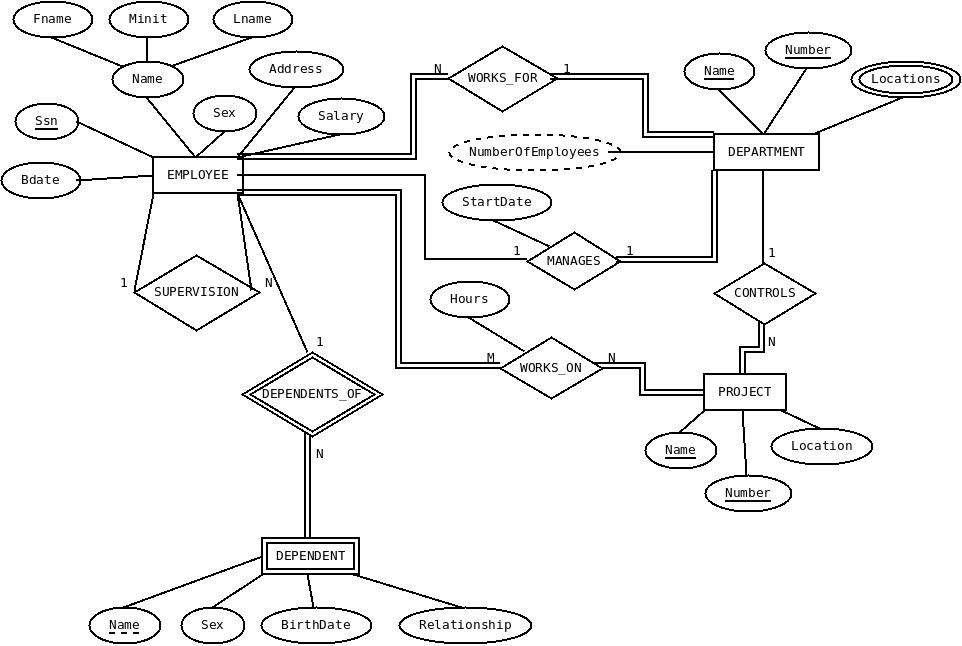
\includegraphics[width=0.6\textwidth]{exemplos/diagramas/ER.jpeg}
    \fonte{Indicar autor original.}
\end{figure}


\begin{figure}
    \centering
    \caption{Exemplo de diagrama - salvo imagem vetorizada - EPS}
    \label{fig:uml_dia_vetorizado_eps}
	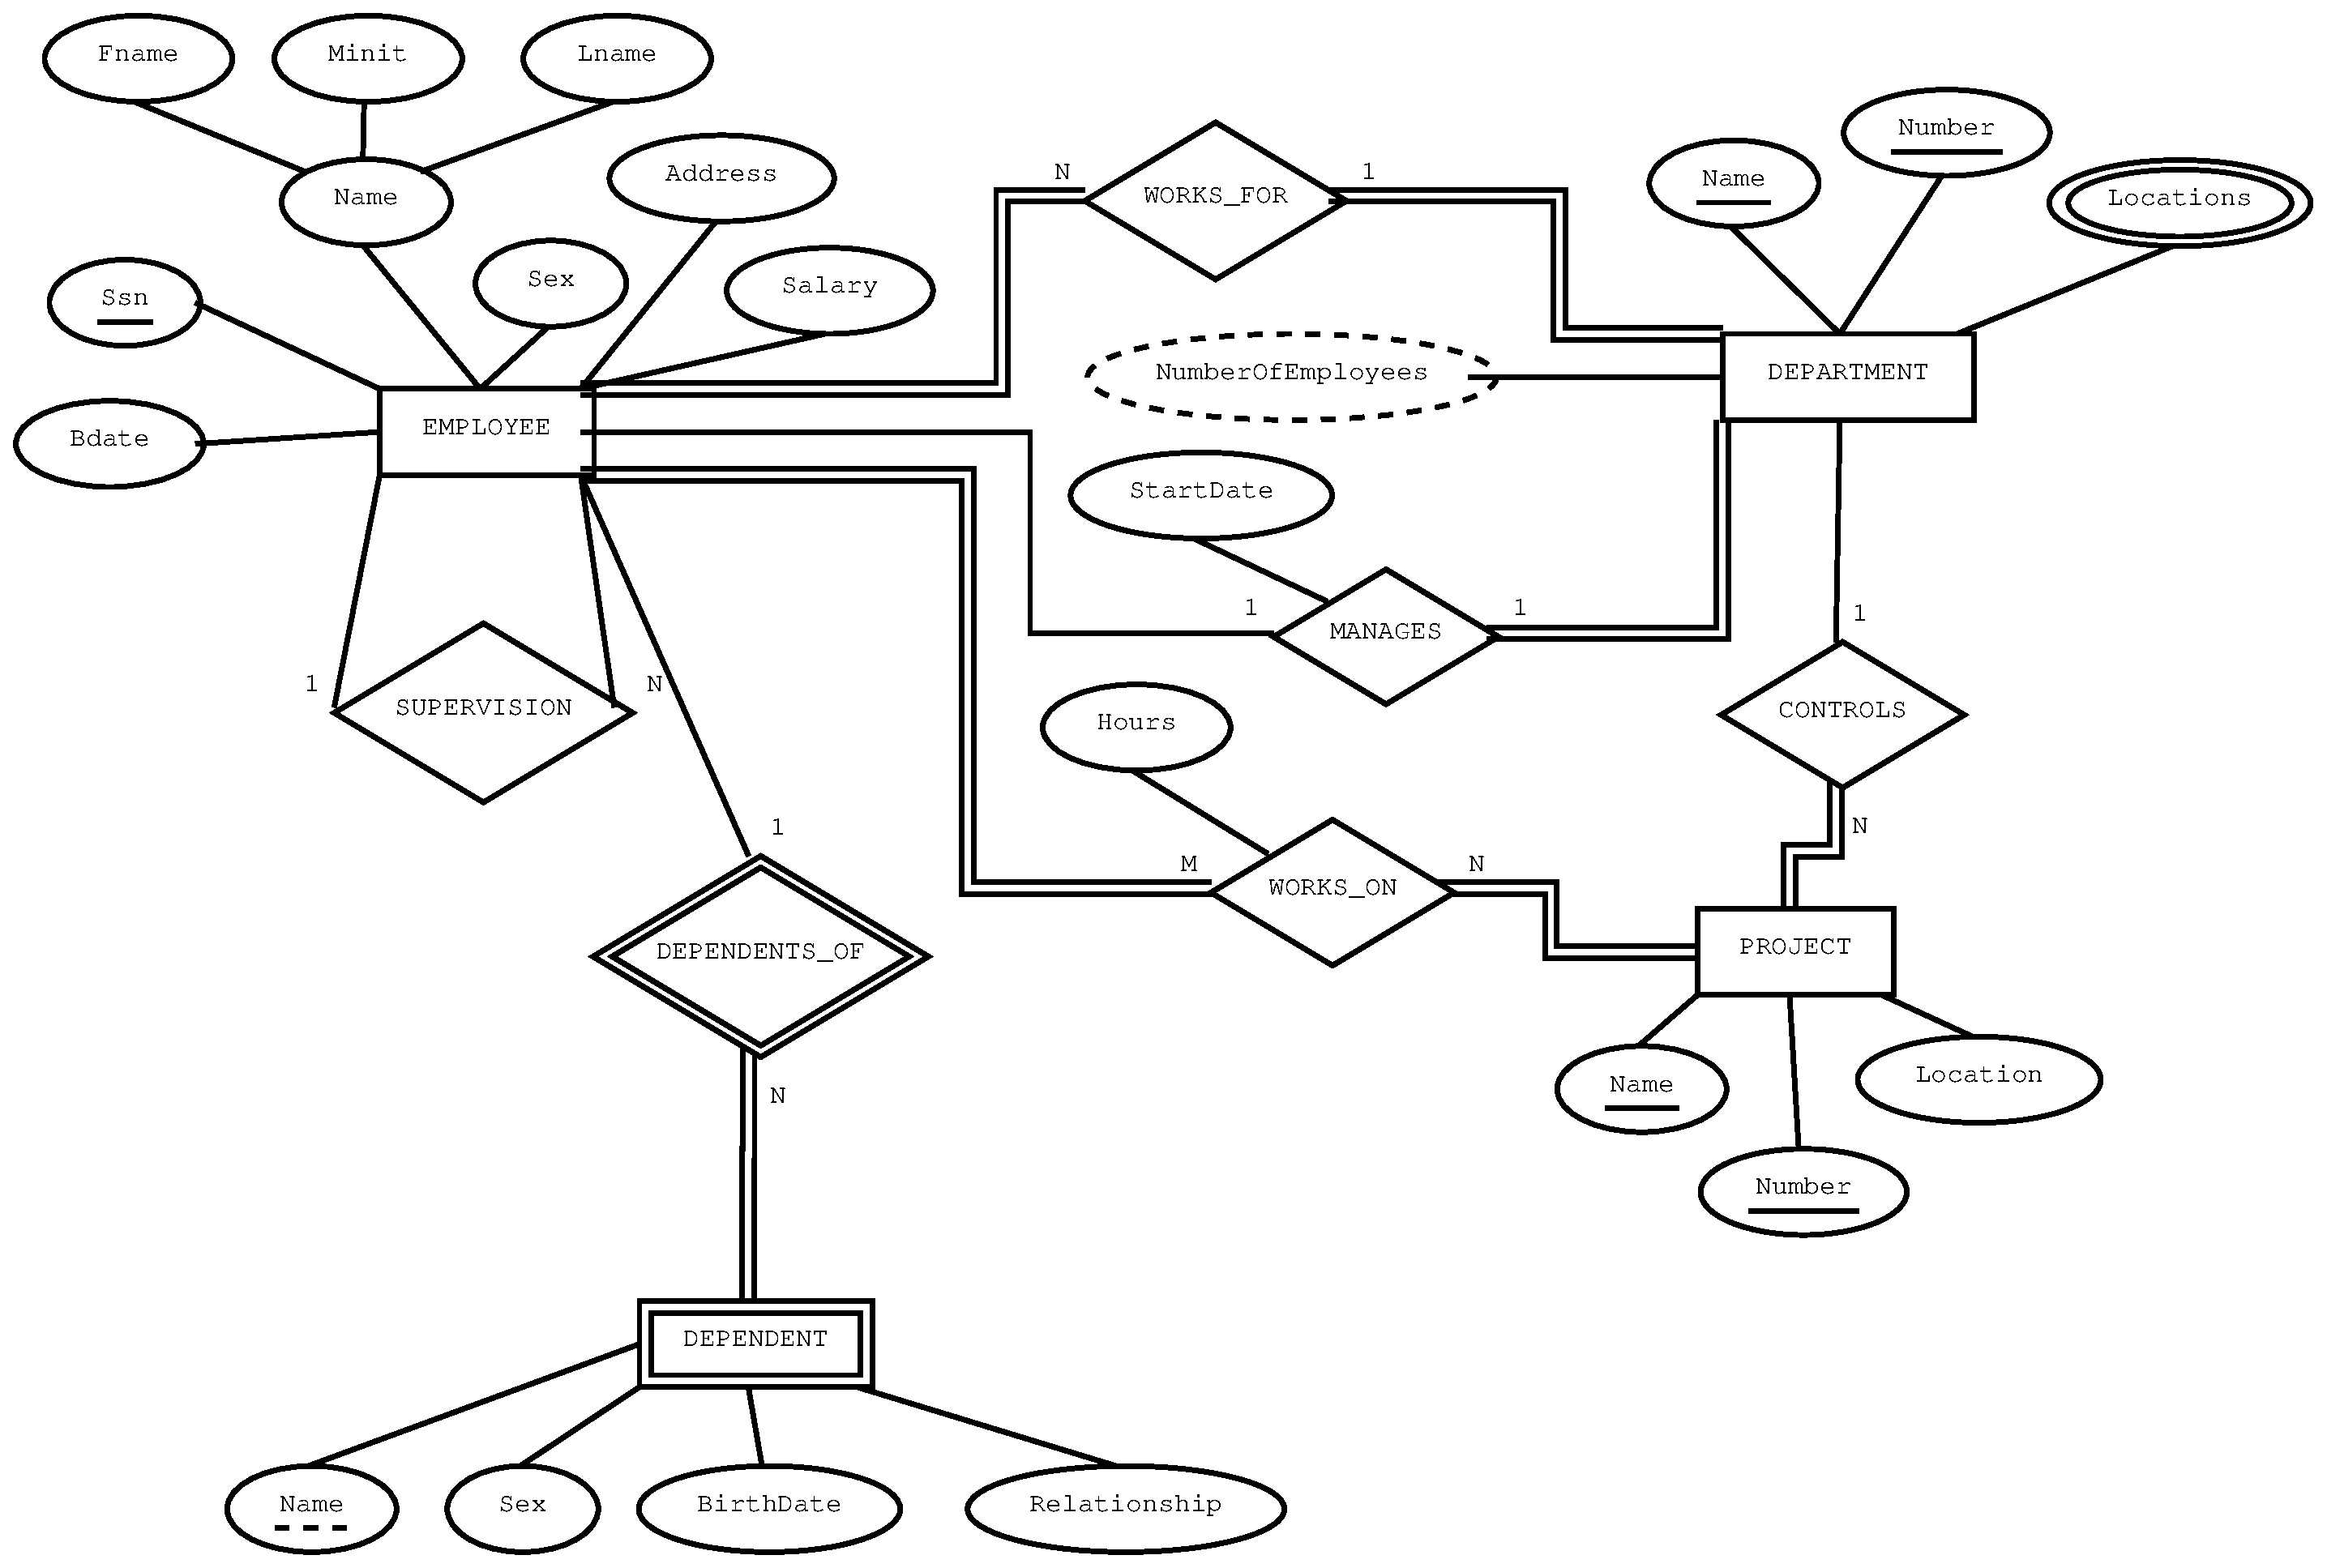
\includegraphics[width=0.6\textwidth]{exemplos/diagramas/ER.eps}
    \fonte{Indicar autor original.}
\end{figure}

\begin{figure}
    \centering
    \caption{Exemplo de diagrama - salvo imagem vetorizada - SVG}
    \label{fig:uml_dia_vetorizado_svg}
    \includesvg[inkscapelatex=false,width=0.6\textwidth]{exemplos/diagramas/ER.svg}
    \fonte{Indicar autor original.}
\end{figure}



% generated by Plantuml 7997beta
\definecolor{plantucolor0000}{RGB}{254,254,206}
\definecolor{plantucolor0001}{RGB}{168,0,54}
\definecolor{plantucolor0002}{RGB}{173,209,178}
\definecolor{plantucolor0003}{RGB}{0,0,0}
\definecolor{plantucolor0004}{RGB}{0,0,255}

\begin{figure}[htb]
    \centering
    \caption{\label{diagramauml}Exemplo de Diagrama UML gerado a partir do PlantUML}
\begin{tikzpicture}[yscale=-1]
\draw[color=plantucolor0001,fill=plantucolor0000,line width=1.5pt] (131pt,29pt) rectangle (223pt,90.8359pt);
\draw[color=plantucolor0001,fill=plantucolor0002,line width=1.0pt] (146pt,45pt) ellipse (11pt and 11pt);
\draw[color=black,fill=black] (148.7656pt,40.875pt) ..controls (148.9219pt,40.6563pt) .. (149.1094pt,40.5469pt) ..controls (149.2969pt,40.4375pt) .. (149.5156pt,40.4375pt) ..controls (149.8906pt,40.4375pt) .. (150.125pt,40.6953pt) ..controls (150.3594pt,40.9531pt) .. (150.3594pt,41.5625pt) -- (150.3594pt,43.0156pt) ..controls (150.3594pt,43.625pt) .. (150.125pt,43.8906pt) ..controls (149.8906pt,44.1563pt) .. (149.5156pt,44.1563pt) ..controls (149.1719pt,44.1563pt) .. (148.9688pt,43.9531pt) ..controls (148.7656pt,43.7656pt) .. (148.6563pt,43.25pt) ..controls (148.6094pt,42.8906pt) .. (148.4219pt,42.7031pt) ..controls (148.0938pt,42.3281pt) .. (147.4844pt,42.1094pt) ..controls (146.875pt,41.8906pt) .. (146.25pt,41.8906pt) ..controls (145.4844pt,41.8906pt) .. (144.8516pt,42.2188pt) ..controls (144.2188pt,42.5469pt) .. (143.7266pt,43.2969pt) ..controls (143.2344pt,44.0469pt) .. (143.2344pt,45.0781pt) -- (143.2344pt,46.1719pt) ..controls (143.2344pt,47.4063pt) .. (144.125pt,48.2266pt) ..controls (145.0156pt,49.0469pt) .. (146.6094pt,49.0469pt) ..controls (147.5469pt,49.0469pt) .. (148.2031pt,48.7969pt) ..controls (148.5938pt,48.6406pt) .. (149.0156pt,48.2031pt) ..controls (149.2813pt,47.9375pt) .. (149.4297pt,47.8594pt) ..controls (149.5781pt,47.7813pt) .. (149.7813pt,47.7813pt) ..controls (150.1094pt,47.7813pt) .. (150.3672pt,48.0391pt) ..controls (150.625pt,48.2969pt) .. (150.625pt,48.6406pt) ..controls (150.625pt,48.9844pt) .. (150.2813pt,49.3906pt) ..controls (149.7813pt,49.9688pt) .. (148.9844pt,50.2969pt) ..controls (147.9063pt,50.75pt) .. (146.6094pt,50.75pt) ..controls (145.0938pt,50.75pt) .. (143.8906pt,50.125pt) ..controls (142.9063pt,49.625pt) .. (142.2188pt,48.5547pt) ..controls (141.5313pt,47.4844pt) .. (141.5313pt,46.2031pt) -- (141.5313pt,45.0469pt) ..controls (141.5313pt,43.7188pt) .. (142.1484pt,42.5703pt) ..controls (142.7656pt,41.4219pt) .. (143.8594pt,40.8047pt) ..controls (144.9531pt,40.1875pt) .. (146.1875pt,40.1875pt) ..controls (146.9219pt,40.1875pt) .. (147.5703pt,40.3516pt) ..controls (148.2188pt,40.5156pt) .. (148.7656pt,40.875pt);
\node at (160pt,37.4531pt)[below right]{Subscriber};
\draw[color=plantucolor0001,line width=1.5pt] (132pt,61pt) -- (222pt,61pt);
\node at (137pt,65pt)[below right]{subscriberId};
\draw[color=plantucolor0001,line width=1.5pt] (132pt,82.8359pt) -- (222pt,82.8359pt);
\draw[color=plantucolor0001,fill=plantucolor0000,line width=1.5pt] (31pt,212pt) rectangle (137pt,273.8359pt);
\draw[color=plantucolor0001,fill=plantucolor0002,line width=1.0pt] (46pt,228pt) ellipse (11pt and 11pt);
\draw[color=black,fill=black] (48.7656pt,223.875pt) ..controls (48.9219pt,223.6563pt) .. (49.1094pt,223.5469pt) ..controls (49.2969pt,223.4375pt) .. (49.5156pt,223.4375pt) ..controls (49.8906pt,223.4375pt) .. (50.125pt,223.6953pt) ..controls (50.3594pt,223.9531pt) .. (50.3594pt,224.5625pt) -- (50.3594pt,226.0156pt) ..controls (50.3594pt,226.625pt) .. (50.125pt,226.8906pt) ..controls (49.8906pt,227.1563pt) .. (49.5156pt,227.1563pt) ..controls (49.1719pt,227.1563pt) .. (48.9688pt,226.9531pt) ..controls (48.7656pt,226.7656pt) .. (48.6563pt,226.25pt) ..controls (48.6094pt,225.8906pt) .. (48.4219pt,225.7031pt) ..controls (48.0938pt,225.3281pt) .. (47.4844pt,225.1094pt) ..controls (46.875pt,224.8906pt) .. (46.25pt,224.8906pt) ..controls (45.4844pt,224.8906pt) .. (44.8516pt,225.2188pt) ..controls (44.2188pt,225.5469pt) .. (43.7266pt,226.2969pt) ..controls (43.2344pt,227.0469pt) .. (43.2344pt,228.0781pt) -- (43.2344pt,229.1719pt) ..controls (43.2344pt,230.4063pt) .. (44.125pt,231.2266pt) ..controls (45.0156pt,232.0469pt) .. (46.6094pt,232.0469pt) ..controls (47.5469pt,232.0469pt) .. (48.2031pt,231.7969pt) ..controls (48.5938pt,231.6406pt) .. (49.0156pt,231.2031pt) ..controls (49.2813pt,230.9375pt) .. (49.4297pt,230.8594pt) ..controls (49.5781pt,230.7813pt) .. (49.7813pt,230.7813pt) ..controls (50.1094pt,230.7813pt) .. (50.3672pt,231.0391pt) ..controls (50.625pt,231.2969pt) .. (50.625pt,231.6406pt) ..controls (50.625pt,231.9844pt) .. (50.2813pt,232.3906pt) ..controls (49.7813pt,232.9688pt) .. (48.9844pt,233.2969pt) ..controls (47.9063pt,233.75pt) .. (46.6094pt,233.75pt) ..controls (45.0938pt,233.75pt) .. (43.8906pt,233.125pt) ..controls (42.9063pt,232.625pt) .. (42.2188pt,231.5547pt) ..controls (41.5313pt,230.4844pt) .. (41.5313pt,229.2031pt) -- (41.5313pt,228.0469pt) ..controls (41.5313pt,226.7188pt) .. (42.1484pt,225.5703pt) ..controls (42.7656pt,224.4219pt) .. (43.8594pt,223.8047pt) ..controls (44.9531pt,223.1875pt) .. (46.1875pt,223.1875pt) ..controls (46.9219pt,223.1875pt) .. (47.5703pt,223.3516pt) ..controls (48.2188pt,223.5156pt) .. (48.7656pt,223.875pt);
\node at (60pt,220.4531pt)[below right]{AccumUsage};
\draw[color=plantucolor0001,line width=1.5pt] (32pt,244pt) -- (136pt,244pt);
\node at (37pt,248pt)[below right]{subscriberId};
\draw[color=plantucolor0001,line width=1.5pt] (32pt,265.8359pt) -- (136pt,265.8359pt);
\draw[color=plantucolor0001,fill=plantucolor0000,line width=1.5pt] (221pt,191pt) rectangle (318pt,294.3438pt);
\draw[color=plantucolor0001,fill=plantucolor0002,line width=1.0pt] (240.05pt,207pt) ellipse (11pt and 11pt);
\draw[color=black,fill=black] (242.8156pt,202.875pt) ..controls (242.9719pt,202.6563pt) .. (243.1594pt,202.5469pt) ..controls (243.3469pt,202.4375pt) .. (243.5656pt,202.4375pt) ..controls (243.9406pt,202.4375pt) .. (244.175pt,202.6953pt) ..controls (244.4094pt,202.9531pt) .. (244.4094pt,203.5625pt) -- (244.4094pt,205.0156pt) ..controls (244.4094pt,205.625pt) .. (244.175pt,205.8906pt) ..controls (243.9406pt,206.1563pt) .. (243.5656pt,206.1563pt) ..controls (243.2219pt,206.1563pt) .. (243.0188pt,205.9531pt) ..controls (242.8156pt,205.7656pt) .. (242.7063pt,205.25pt) ..controls (242.6594pt,204.8906pt) .. (242.4719pt,204.7031pt) ..controls (242.1438pt,204.3281pt) .. (241.5344pt,204.1094pt) ..controls (240.925pt,203.8906pt) .. (240.3pt,203.8906pt) ..controls (239.5344pt,203.8906pt) .. (238.9016pt,204.2188pt) ..controls (238.2688pt,204.5469pt) .. (237.7766pt,205.2969pt) ..controls (237.2844pt,206.0469pt) .. (237.2844pt,207.0781pt) -- (237.2844pt,208.1719pt) ..controls (237.2844pt,209.4063pt) .. (238.175pt,210.2266pt) ..controls (239.0656pt,211.0469pt) .. (240.6594pt,211.0469pt) ..controls (241.5969pt,211.0469pt) .. (242.2531pt,210.7969pt) ..controls (242.6438pt,210.6406pt) .. (243.0656pt,210.2031pt) ..controls (243.3313pt,209.9375pt) .. (243.4797pt,209.8594pt) ..controls (243.6281pt,209.7813pt) .. (243.8313pt,209.7813pt) ..controls (244.1594pt,209.7813pt) .. (244.4172pt,210.0391pt) ..controls (244.675pt,210.2969pt) .. (244.675pt,210.6406pt) ..controls (244.675pt,210.9844pt) .. (244.3313pt,211.3906pt) ..controls (243.8313pt,211.9688pt) .. (243.0344pt,212.2969pt) ..controls (241.9563pt,212.75pt) .. (240.6594pt,212.75pt) ..controls (239.1438pt,212.75pt) .. (237.9406pt,212.125pt) ..controls (236.9563pt,211.625pt) .. (236.2688pt,210.5547pt) ..controls (235.5813pt,209.4844pt) .. (235.5813pt,208.2031pt) -- (235.5813pt,207.0469pt) ..controls (235.5813pt,205.7188pt) .. (236.1984pt,204.5703pt) ..controls (236.8156pt,203.4219pt) .. (237.9094pt,202.8047pt) ..controls (239.0031pt,202.1875pt) .. (240.2375pt,202.1875pt) ..controls (240.9719pt,202.1875pt) .. (241.6203pt,202.3516pt) ..controls (242.2688pt,202.5156pt) .. (242.8156pt,202.875pt);
\node at (254.95pt,199.4531pt)[below right]{IpSession};
\draw[color=plantucolor0001,line width=1.5pt] (222pt,223pt) -- (317pt,223pt);
\node at (227pt,227pt)[below right]{ipAddress};
\node at (227pt,240.8359pt)[below right]{specificData};
\node at (227pt,254.6719pt)[below right]{sapcOriginStateId};
\node at (227pt,268.5078pt)[below right]{apnId};
\draw[color=plantucolor0001,line width=1.5pt] (222pt,286.3438pt) -- (317pt,286.3438pt);
\draw[color=plantucolor0004] (191.942pt,90.081pt) ..controls (205.204pt,115.893pt) and (224.952pt,154.325pt) .. (241.265pt,186.076pt);
\draw[color=plantucolor0004,fill=plantucolor0004] (243.646pt,190.709pt) -- (243.0894pt,180.8759pt) -- (241.3604pt,186.262pt) -- (235.9742pt,184.5329pt) -- (243.646pt,190.709pt) -- cycle;
\node at (191.0584pt,98.9168pt)[below right]{1};
\node at (230.3817pt,166.6703pt)[below right]{1..*};
\draw[color=plantucolor0001] (162.058pt,90.081pt) ..controls (145.645pt,122.023pt) and (119.302pt,173.295pt) .. (101.824pt,207.31pt);
\draw[color=plantucolor0001,fill=plantucolor0001] (99.5252pt,211.784pt) -- (107.1969pt,205.6078pt) -- (101.8108pt,207.337pt) -- (100.0816pt,201.9509pt) -- (99.5252pt,211.784pt) -- cycle;
\node at (143.0082pt,98.7264pt)[below right]{1};
\node at (101.801pt,187.522pt)[below right]{0..1};
\end{tikzpicture}
	\legend{Fonte: Exemplos PlantUML.}
\end{figure}

A \autoref{fig_diag_virado} exemplifica como utilizar uma imagem em formato paisagem (página inteira). Obs: Utilizamos propositalmente uma imagem não vetorizada de forma a ilustrar o procedimento e também para apresentar que a qualidade não fica boa o suficiente para leitura. Uma versão vetorizada dessa figura teria qualidade melhor.


% observe que a imagem a seguir teve que ser ajustada para caber corretamente na página
% por não ser uma imagem vetorizada a qualidade não é a melhor possivel
\begin{sidewaysfigure}[htb]
    \centering
	\caption{\label{fig_diag_virado}Diagrama Virado - Exemplo}
	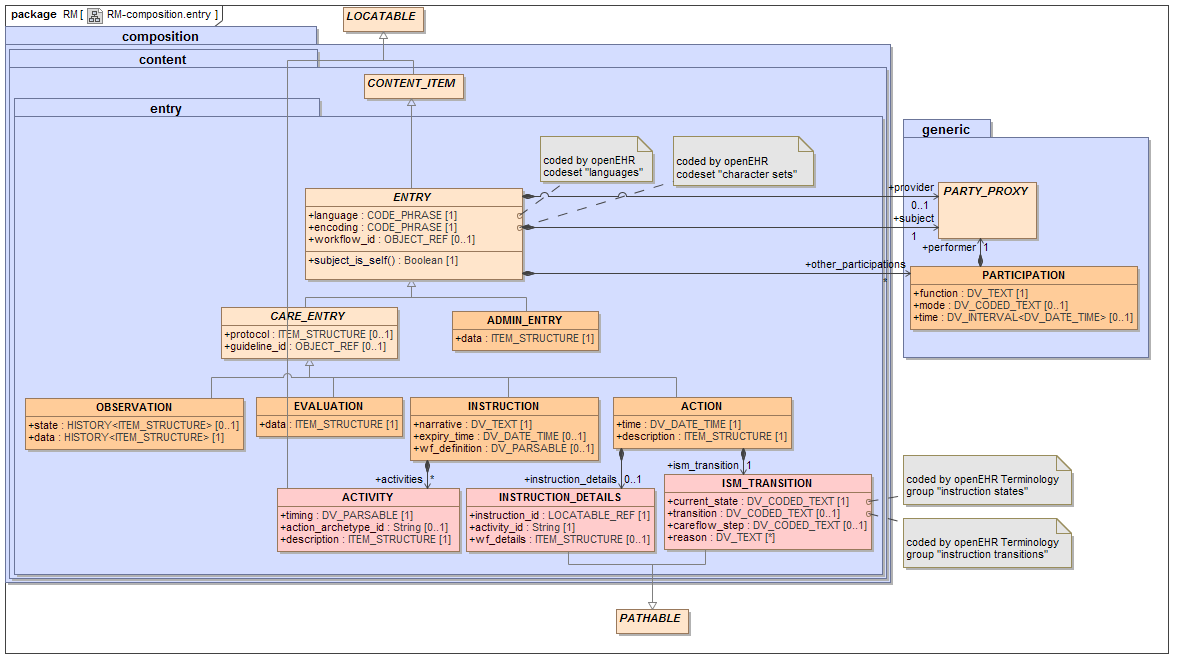
\includegraphics[width=0.9\textwidth]{exemplos/exemplo_diag_horizontal.png}
	\fonte{\citeonline{openehrCompositionEntry}.}
\end{sidewaysfigure}


\subsection{Impressão em folhas formato A3}

A página seguinte em A3 permite a impressão de diagramas grandes que não podem ser visualizados facilmente em folha padrão A4. Lembre que algumas impressoras podem ter problemas com isso, então selecione somente as páginas A4 ao imprimir e depois imprima separadamente a página A3.

A \autoref{fig_logo_A3} utiliza a mesma imagem da \autoref{fig_logo} e foi ampliada para demonstrar a essa possibilidade de impressão de grandes imagens em A3.

Observe que o código de exemplo vai gerar uma quebra de página no local onde for definida a página A3, por isso não deve ser utilizado entre textos para evitar grandes espaços em branco.

Folhas impressas em A3 ou tamanhos maiores devem ser dobradas seguindo o padrão definido pela \ac{abnt}. 


Cuidado ao utilizar folhas A3 em um documento impresso em frente e verso pois a numeração das páginas seguintes pode ser impressa de forma incorreta (posição do número na página). Uma alternativa para esta situação é manter todas páginas impressas em A3 no último apêndice, fazendo as referencias corretas durante o texto.



 \afterpage{%
 \begin{PAGINA-A3}

 \begin{figure}[p]
     \centering%
 	\caption{\label{fig_logo_A3}Logotipo \acs{ifsp} em página A3}
     \fcolorbox{red}{yellow}{ 
\includegraphics[height=\textheight,width=\textwidth,keepaspectratio]{\ifspprefixo/logo-02.jpg}}%
 	\legend{Com borda para demonstrar os limites}
   \fonte{citar o autor da Figura(xxx).}
 \end{figure}

 \end{PAGINA-A3}
 }





% ---
% Conclusão (outro exemplo de capítulo sem numeração e presente no sumário)
% Dependendo do trabalho desenvolvido ele pode ter uma Conclusão ou Considerações finais
% Para trabalhos de disciplina utilizar Considerações Finais
% ---
\chapter{Considerações Finais}

Esse capítulo tem como intuito descrever o desenvolvimento da aplicação feita pela equipe, demonstrando as dificuldades no decorrer do projeto. Como também informando as lições aprendidas com essa experiência.

\section{Principais Dificuldades}
Desde o início do projeto, foi compreendido pelos componentes que não seria um trabalho fácil, seria necessário auto-disciplina, dedicação  e principalmente, o apoio coletivo da equipe. De maneira inicial, foi difícil, visto que a equipe encontrava-se em níveis diferentes de conhecimento e desenvolvimento. \\
 No início, a dificuldade encontrada, ocorreu quando os integrantes da equipe tinham tempo limitado para o desenvolvimento do projeto. Os integrantes trabalham em tempo integral, fazendo com que, o único tempo disponível seria de noite ou finais de semana. Mesmo reorganizando as funções, cada integrante não teria muito tempo para realizar as funções destinadas a cada um. \\
Imprevistos aconteceram durante a semana, onde interferiu diretamente no projeto. Desse jeito, dois integrantes do grupo saíram, o Kelvin e o Lucas, aumentando a carga de trabalho e a responsabilidade de todos.\\
A segunda dificuldade ocorreu quando os integrantes informaram que teriam conhecimentos básicos com as tecnologias utilizadas, como React Native, PostgreSQL, Expo, etc. Nem todos possuíam uma grande curva de aprendizado e, devido a pouca disponibilidade, isso acabou atrapalhando o desenvolvimento do projeto. Como tentativa de amenizar esse problema, realizamos algumas videochamadas para nos ajudarmos.\\


\section{Lições Aprendidas}
Ao decorrer do projeto, a equipe observou que teria que se comunicar melhor sobre o projeto, para evitar retrabalhos, pois com a falta dessa comunicação fez com que alguns tópicos fossem refeitos como, os Casos de Uso, MER, DER, etc.\\
Os Wireframes passaram a ser refeitos no decorrer do projeto, por conta das correções de funcionalidades do usuário. \\
Após identificar os pontos de melhoria, as mudanças nos padrões de comportamento trouxeram muito mais união à equipe. Observaram-se muitos pontos positivos durante o desenvolvimento, relacionados à empatia, paciência  e esforço de cada integrante durante o trabalho. Desta forma, a equipe teve uma melhora muito grande ao final do projeto. \\


\section{Funcionalidades Futuras}
Por se tratar de um aplicativo de transporte, o projeto tem potencial para ter grandes mudanças no decorrer do tempo e das necessidades que vão aparecer, de melhoria e atualizações que podem abranger leis e normas públicas, como novas funcionalidades para usuários, de modo que o App se torne mais atrativo para os usuário e futuras parcerias. Por exemplo, a inclusão de transporte de Pets usando aviões em viagens nacionais como internacionais.\\
Para o futuro, buscamos ter grande aproveitamento no crescimento do aplicativo para uso não só em território nacional como internacional, gerando assim questões como mais idiomas para o aplicativo, usar servidores externos ou até mesmo parcerias fora do Brasil.\\
Visando o cliente final, é desejado ter uma interface mais simples visando pessoas idosas ou que não possuem grande conhecimento em tecnologia usando aplicativos.\\



% ----------------------------------------------------------
% Finaliza a parte no bookmark do PDF
% para que se inicie o bookmark na raiz
% e adiciona espaço de parte no Sumário
% ----------------------------------------------------------
\phantompart

% ----------------------------------------------------------
% ELEMENTOS PÓS-TEXTUAIS
% ----------------------------------------------------------
\postextual
% ----------------------------------------------------------

% ----------------------------------------------------------
% Referências bibliográficas
% ----------------------------------------------------------
\bibliography{referencias,exemplos/abntex2-doc-abnt-6023}

% ----------------------------------------------------------
% Glossário
% ----------------------------------------------------------
%
%
\ifdef{\printnoidxglossary}{
    \addcontentsline{toc}{chapter}{GLOSSÁRIO}
    \printnoidxglossary[style=glossario]
    %\printglossaries
}{}

% ----------------------------------------------------------
% Apêndices
% Documentos gerados pelo próprio autor
% ----------------------------------------------------------

% ---
% Inicia os apêndices
% ---
\begin{apendicesenv}

% Imprime uma página indicando o início dos apêndices
\partapendices

% ----------------------------------------------------------
\chapter{QUESTÃO DE PESQUISA}
% ----------------------------------------------------------

\subsection{Como os animais são transportados ?}
\label{p1}
\subsection{Como solicitar uma viagem ?}
\label{p2}
\subsection{Como será a higienização do carro?}
\label{p3}
\subsection{O aplicativo irá permitir quantos animais no carro ?}
\label{p4}
\subsection{O aplicativo terá agendamentos ?}
\label{p5}
\subsection{Será possível, que o animal viaje sem o seu dono ?}
\label{p6}
\subsection{Teremos parcerias ?}
\label{p7}
\subsection{Como serão os métodos de pagamentos e como esse valor será cobrado ?}
\label{p8}
\subsection{Como será a comunicação entre o passageiro e o motorista ?}
\label{p9}
\subsection{Como será o método de contratação do motorista ?}
\label{p10}
\subsection{Como será o método de avaliação do motorista ?}
\label{p11}
\subsection{Como será o benefício comum e o premium ?}
\label{p12}
\subsection{Como será o histórico de corridas ?}
\label{p13}
\subsection{Quais animais serão permitidos ?}
\label{p14}
\subsection{Será cobrado alguma taxa extra aos passageiros, para os condutores conseguirem realizar a manutenção no carro a cada viagem ?}
\label{p15}
\subsection{Como será definida a rota de transporte ?}
\label{p16}
\subsection{Como será o chat durante a corrida ?}
\label{p17}
\subsection{Como funcionará o sistema de pontos fidelidade ?}
\label{p18}
\subsection{Como vai funcionar a compra de descontos (Sistemas de pontos)  ?}\label{p19}

\section{Respostas }\\
\subsection{Resposta da pergunta \ref{p1}}
No Carrara Pets, para garantir a segurança e o conforto aos animais, cães usam um cinto de segurança especial que prende no gancho da coleira, e os gatos são transportados dentro de uma caixa específica. Os veículos são higienizados ao final de cada viagem. Caso o pet realize a viagem sozinho, a plataforma envia um SMS automático ao usuário que a corrida foi finalizada, mas também é possível acompanhar o percurso em tempo real por meio do aplicativo. Com o aplicativo, é possível acompanhar a viagem em tempo real, e o pagamento é feito pelo aplicativo.

\subsection{Resposta da pergunta \ref{p2}}
Para solicitar uma corrida, basta abrir o aplicativo e informar os locais de encontro e de destino. O usuário pode acompanhar o trajeto em tempo real, e também consegue realizar o agendamento de corridas. O pagamento pode ser feito com cartão de crédito, a um preço fixo. Com o objetivo de garantir um bom atendimento, é possível visualizar a avaliação dos motoristas, feita por outros usuários da plataforma.

\subsection{Resposta da pergunta \ref{p3}}
Todos os veículos estarão equipados com Kit de proteção que inclui guia, cinto peitoral e focinheira para cães. No caso dos gatos, conectamos a sua caixa de transporte própria ao nosso sistema de segurança. A higiene do veículo também é bastante cuidadosa. Os bancos possuem uma capa protetora de assento, que são aspiradas ao final de cada corrida e recebem uma solução fungicida (combate fungos), viricida (inibe a proliferação de um vírus num processo infeccioso) e bactericida (antibióticos que destroem bactérias) de uso veterinário. É um processo muito importante, pois evita disseminação de doenças entre os animais e humanos também, além de deixar o carro limpo para a próxima corrida.

\subsection{Resposta da pergunta \ref{p4}}
No aplicativo iremos possuir um campo específico para informar a quantidade de pets que irão viajar no veículo e os portes dos animais. 
\textbf{Regras:} 
\begin{itemize}
    \item 1 animal - porte grande, médio ou pequeno.
    \item 2 animais - porte grande e um médio 
    \item 3 animais - porte médio e pequeno 
    \item 4 animais - porte pequeno.
\end{itemize} 

\subsection{Resposta da pergunta \ref{p5}}
Sim. Você contará com a comodidade de agendamento prévio de corridas. Funciona do seguinte modo: você seleciona o dia, a hora e o local para o nosso motorista ir buscar o seu pet e você no local solicitado.

\subsection{Resposta da pergunta \ref{p6}}
Sim. Você poderá realizar o despacho do seu pet desacompanhado. Você não vai precisar acompanhá-lo na viagem se não puder ou quiser, basta ter um responsável para entregar o animal ao motorista no local de origem e outro para receber no local de destino. 
\textit{Pontos Negativos com o serviço de transportes de passageiros ou públicos para deslocar com o seu pet:}
\begin{enumerate}
    \item Insegurança - a falta de equipamentos de segurança para prender corretamente o seu pet ao cinto de segurança e a falta de conhecimento do condutos podem causar acidentes.
    \item Desrespeito às normas de trânsito - O código de trânsito brasileiro (CTB) estabelece normas para o transporte dos animais, motoristas que não possuem treinamentos específicos, podem desconhecê-las e acabam transportando o seu cão de forma errada. 
    \item Motorista despreparados - o motorista não tem experiência e nem treinamento para fazer o transporte dos pet. Além disso, podem ficar irritados se o animal fizer sujeira no carro. 
    \item Falta de equipamentos - os veículos comuns não possuem os acessórios de segurança e higiene para pet.
\end{enumerate}

\subsection{Resposta da pergunta \ref{p7}}
Sim. Iremos ter parcerias com estabelecimentos de pet, como Pet Shop, veterinário, Banho e Tosa. Caso a pessoa seja dono ou gestor de um estabelecimento, poderá entrar em contato conosco e pedir os nossos serviços de transporte de animais domésticos à sua empresa.

\subsection{Resposta da pergunta \ref{p8}}
O app permite cadastrar métodos como cartão de crédito ou dinheiro, para que o passageiro possa escolher a melhor maneira de pagar suas corridas.

\subsection{Resposta da pergunta \ref{p9}}
O método de comunicação entre o passageiro e o motorista será através de um chat, onde os dois indivíduos podem se comunicar entre possíveis atrasos, localizações, consultas de veterinários, comportamento do animal.

\subsection{Resposta da pergunta \ref{p10}}
A contratação de um motorista parceiro, será realizada através do próprio aplicativo em uma aba específica para motoristas parceiros “Seja Parceiro”. O processo de cadastro será feito em três etapas, a primeira que seria o pré-cadastro, será preenchido as informações do motorista como Nome, CPF, CNH, telefone, e-mail, idade, endereço, placa e modelo do veículo, se tem pet ou não e uma carta respondendo a seguinte pergunta “Por que deverá ser aceito ?”. Na segunda etapa teremos uma entrevista com um psicólogo e um teste psicanalítico e psicotécnico, e por fim a etapa de confirmação de cadastro, onde o candidato irá receber um email com o resultado.

\subsection{Resposta da pergunta \ref{p11}}
A avaliação do motorista será solicitada ao final de toda corrida, no app do nosso cliente, em formato de pop-up no seguinte modelo : 
\\
    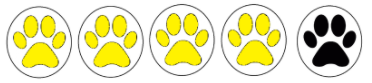
\includegraphics{exemplos/diagramas/star.PNG}
\\
Onde irá de uma “patinha” a cinco “patinhas”.
Obs: Avaliações de uma “patinhas” a duas “patinhas”, após a avaliação será apresentado um campo de texto para incluir observação de um possível problema ou feedback.

\subsection{Resposta da pergunta \ref{p12}}
\textbf{Benefício Comum:}
\begin{itemize}
    \item Apenas transportes.
\end{itemize} 
\textbf{Benefícios para o Premium:}
\begin{itemize}
    \item Aumento no ganho de pontos.
    \item Descontos adquiridos por meio do sistema de pontos, serão dobrados.
    \item Prioridade em motoristas bem avaliados.
\end{itemize}

\subsection{Resposta da pergunta \ref{p13}}
O histórico de corridas será apresentado no ícone “
    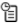
\includegraphics[scale = 0.65]{{exemplos/diagramas/hist.PNG}}
” dentro do aplicativo, e será  composto pelas vinte últimas corridas do cliente. Podendo ter acesso às seguintes informações das corridas : Local de partida, local de destino, rota percorrida, valor da corrida, pet transportado, nome do motorista, modelo e placa do veículo, gastos adicionais (caso tiver), método de pagamento e observações da corrida.

\subsection{Resposta da pergunta \ref{p14}}
Vamos ter uma regra bastante rígida em relação aos pets que poderão ser transportados, onde aceitaremos o cadastro e transporte de somente animais domésticos. Quaisquer tentativas de transporte de animais silvestres serão repudiadas com sujeição a punições.

\subsection{Resposta da pergunta \ref{p15}}
\textbf{Caso tenha a taxa:} 
O nosso aplicativo deixará claro que animais a serviço - como cães-guia, por exemplo - estão isentos de cobrança da taxa, como estipula leis estaduais e federais.

\subsection{Resposta da pergunta \ref{p16}}
O processo de definição será por meio de grafos e informações de trânsito ao vivo, utilizando o ponto de partida e traçando a rota até o ponto de destino, podendo adicionar paradas adicionais.

\subsection{Resposta da pergunta \ref{p17}}
O aplicativo irá contar com um chat durante todas as corridas, onde o motorista e o usuário poderá trocar informações sobre possíveis consultas e detalhes do passeio com o pet, também será possível adicionar documentos (Comprovantes/Diagnósticos) ao chat.

\subsection{Resposta da pergunta \ref{p18}}
Teremos como métodos de fidelidade com o usuário o sistema de pontos, onde ao final de todas as corridas nossos usuários receberão pontos conforme a distância da corrida. O cálculo dos pontos será feito da seguinte forma (distância da viagem em metros) / 10, já para usuários premium o cálculo será ((distância da viagem em metros) / 10) + ((distância da viagem em metros) * 0.04) 
Ex (usuário comum): Viagem de 2,6 km, o usuário receberá 260 pontos.
Ex (usuário premium): Viagem de 2,6km, o usuário receberá 364 pontos.
Esses pontos poderão ser trocados em descontos para viagens futuras.

\subsection{Resposta da pergunta \ref{p19}}
Os valores dos descontos serão :\\
5\% de desconto - 600 pontos.\\
10\% de desconto - 1000 pontos.\\
30\% de desconto - 2800 pontos.\\
50\% de desconto - 4500 pontos.

% ----------------------------------------------------------
\chapter{SPRINTS}
% ----------------------------------------------------------
Essa seção contém o conteúdo desenvolvido durante todas as nossas Sprint(LINK AQUI), separados por onze períodos de uma semana cada reunião. Cara Sprint teve em média duas horas, visando respeitar a disponibilidade dos integrantes do grupo.\\

\begin{figure}
    \centering
    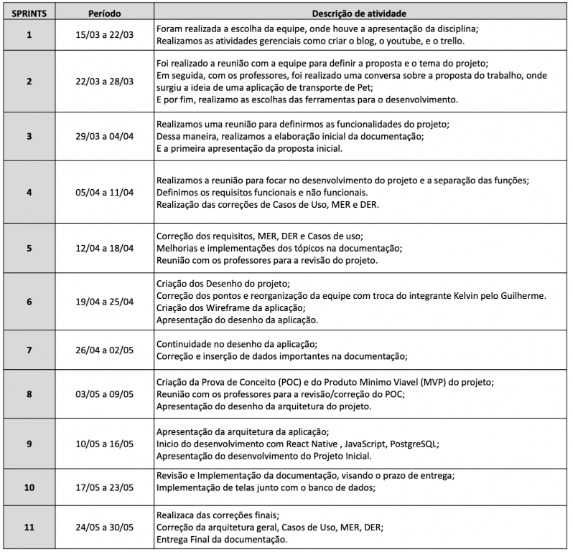
\includegraphics{exemplos/diagramas/Sprints de 11 semanas realizada pela equipe..jpeg}
    \caption{Sprints de 11 semanas realizada pela equipe.}
    \label{fig:Sprints de 11 semanas realizada pela equipe.}
    \fonte {Os Autores}
\end{figure}
% ----------------------------------------------------------
%WIREFRAME
\chapter{Wireframe}
\begin{center}
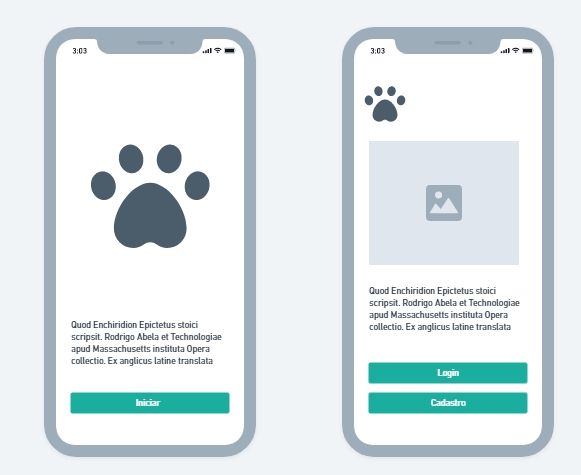
\includegraphics[width=230]{exemplos/Wireframe/Wireframe1.PNG}
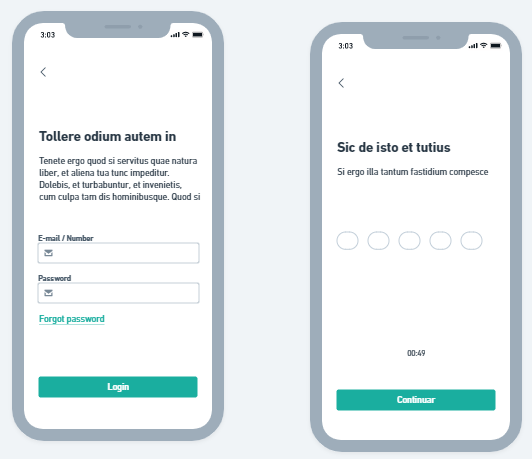
\includegraphics[width=220]{exemplos/Wireframe/Wireframe2.PNG}
\\
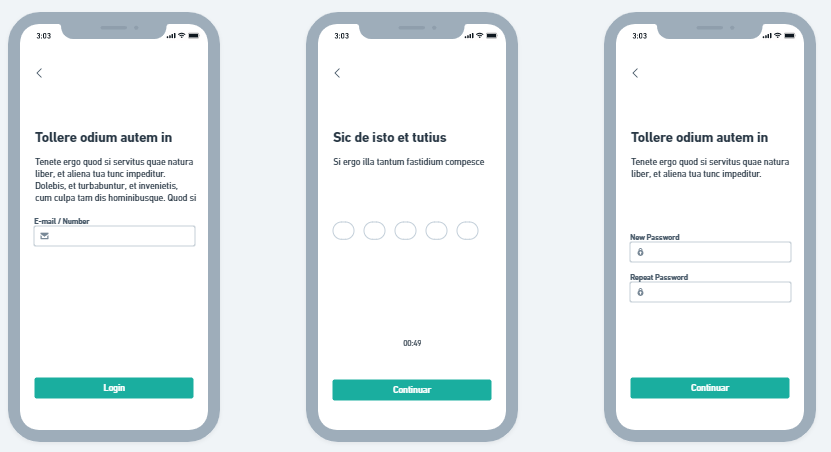
\includegraphics[width=250]{exemplos/Wireframe/Wireframe3.PNG}
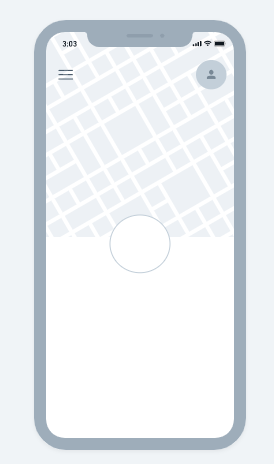
\includegraphics[width=100]{exemplos/Wireframe/Wireframe4.PNG}
\\
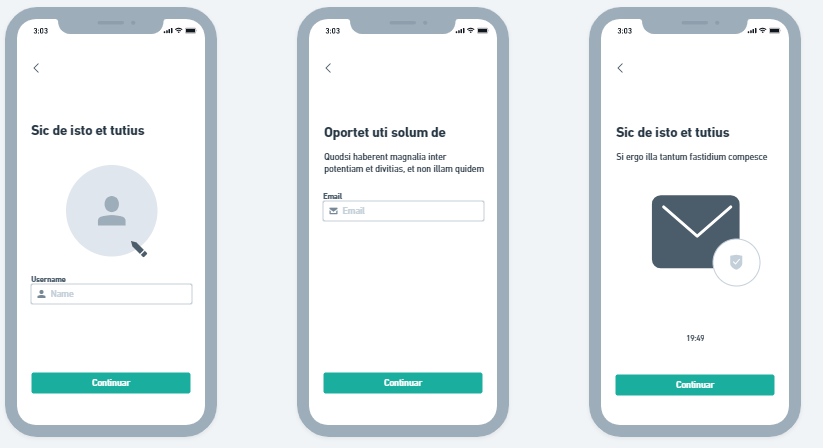
\includegraphics[width=250]{exemplos/Wireframe/Wireframe5.PNG}
\\
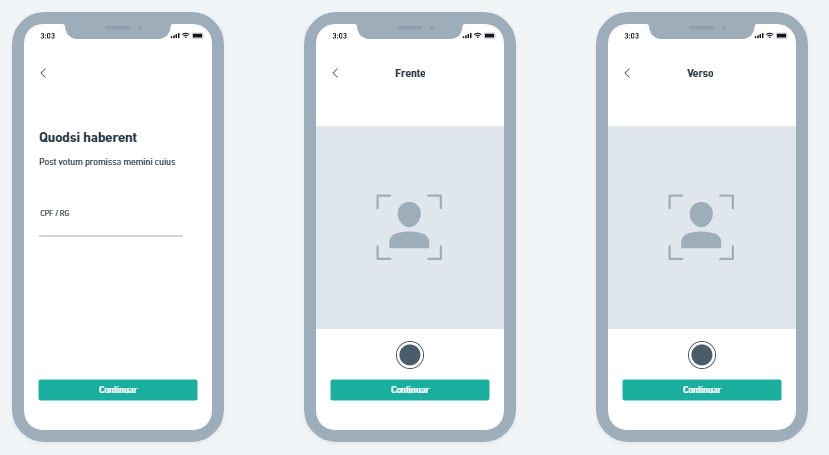
\includegraphics[width=250]{exemplos/Wireframe/Wireframe6.PNG}
\\
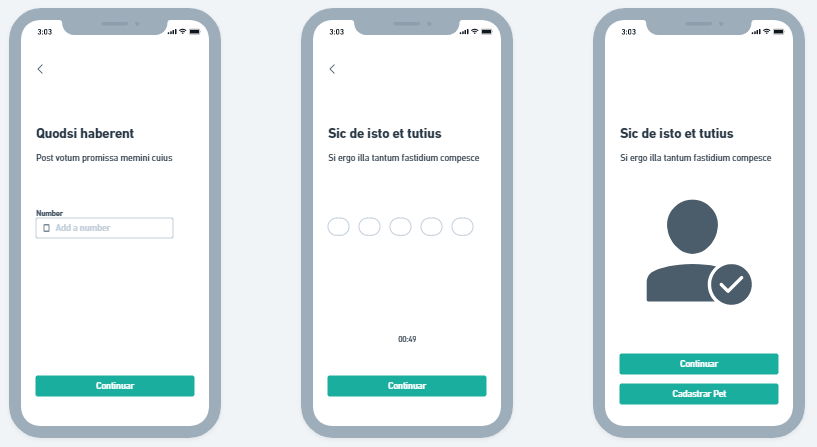
\includegraphics[width=250]{exemplos/Wireframe/Wireframe7.PNG}
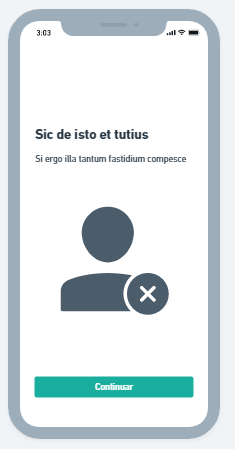
\includegraphics[width=100]{exemplos/Wireframe/Wireframe7_1.PNG}
\\
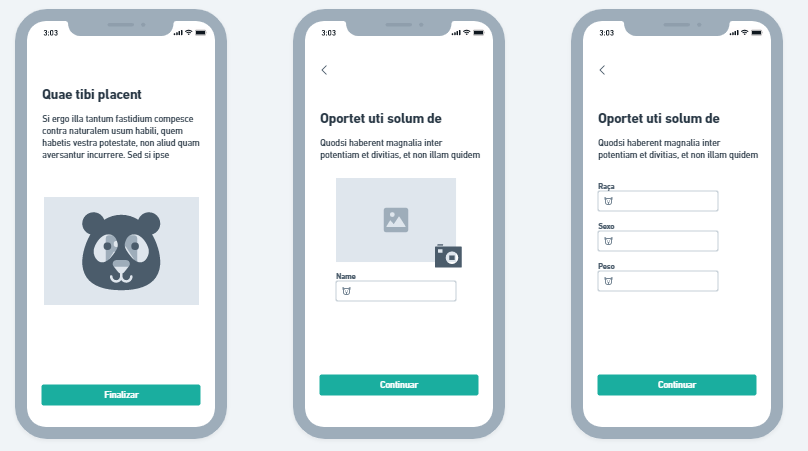
\includegraphics[width=250]{exemplos/Wireframe/Wireframe8.PNG}
\\
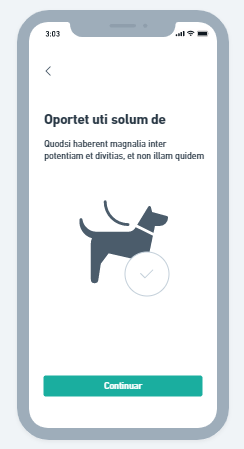
\includegraphics[width=200]{exemplos/Wireframe/Wireframe9.PNG}
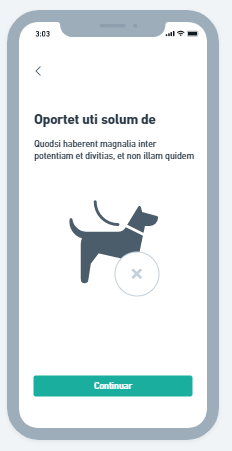
\includegraphics[width=200]{exemplos/Wireframe/Wireframe10.PNG}
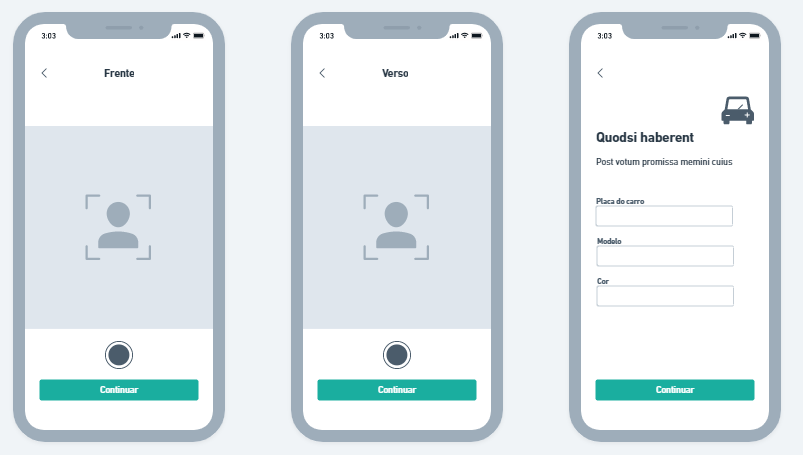
\includegraphics[width=200]{exemplos/Wireframe/Wireframe11.PNG}
\\
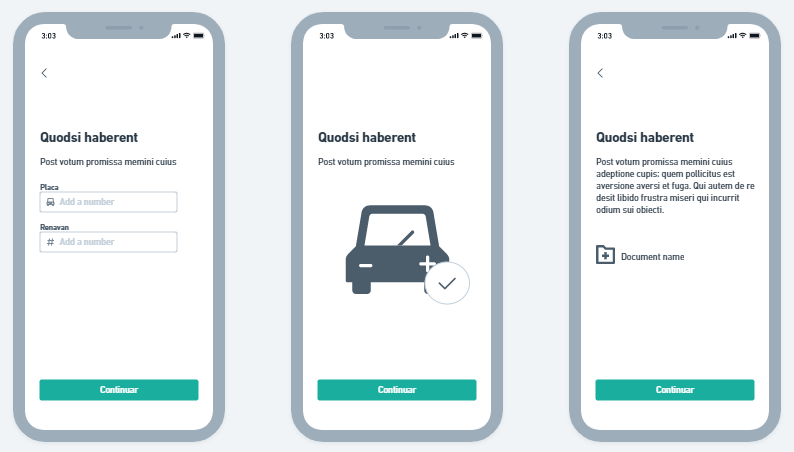
\includegraphics[width=200]{exemplos/Wireframe/Wireframe12.PNG}
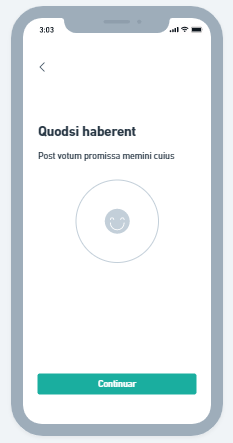
\includegraphics[width=80]{exemplos/Wireframe/Wireframe13.PNG}
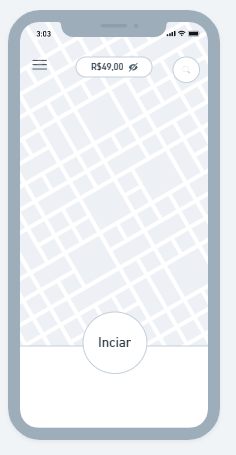
\includegraphics[width=80]{exemplos/Wireframe/Wireframe14.PNG}
\\
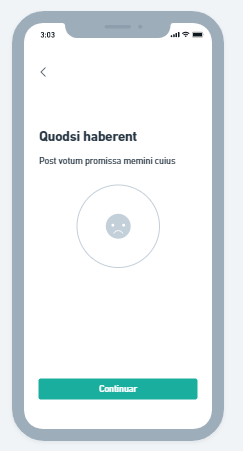
\includegraphics[width=80]{exemplos/Wireframe/Wireframe15.PNG}
\end{center}

% ----------------------------------------------------------
\chapter{HISTÓRIA DE USUÁRIO }
% ----------------------------------------------------------


%REQUISITOS 
\chapter{Requisitos funcionais e não funcionais}

\section{Requisitos funcionais}
\begin{quadro}[thb]
\ABNTEXfontereduzida
\caption{Requisitos Funcionais}
\label{quadro-poluido-limpo-desalinhado}
\begin{tabular}{|l|p{2cm}|l|l|l|p{6cm}|}
\hline
\thead{RF}&\thead{Requisitos\\Funcionais} & \thead{Essencial} & \thead{Importante} & \thead{Desejável} & \thead{Descrição}\\
\hline
RF001&Permitir cadastro de usuários&\circlemark& & & O sistema tem que conceder o cadastro do usuário;\\
\hline
RF002&Permitir cadastro de usuários com conta Google&\circlemark& & & A aplicação deverá permitir que o usuário se cadastre usando a conta Google.\\
\hline
RF003&Permitir cadastro dos Pets&\circlemark& & & O sistema carece que o usuário realize o cadastro do pet (cachorro ou gato).\\
\hline
RF004&Permitir o cadastro do motorista&\circlemark& & & O app deverá aceitar o cadastro do motorista;\\
\hline
RF005&Validar e-mail&\circlemark& & & A aplicação precisa validar se o e-mail informado está correto, enviando um e-mail para o tipo usuário que está solicitando o cadastro. No máximo em 10 segundos.\\
\hline
RF006&Validar celular&\circlemark& & & A aplicação deve enviar um sms validando o número do celular do cliente cadastrado e do motorista no máximo em 10 segundos.\\
\hline
RF007&Realizar o login &\circlemark& & & O sistema deverá permitir o usuário efetuar login;\\
\hline
RF008&Escolher modalidade&\circlemark& & & Quando o cliente acessar o aplicativo o cliente escolher a modalidade comum ou premium, sendo a modalidade comum somente transporte de levar até um local específico e a premium disponibiliza serviços como: transporte e cuidado em parque, acompanhamento no veterinário e etc.\\
\hline
RF009&Quantidade de pets&\circlemark& & & A aplicação deverá solicitar que o cliente informe a quantidade de pets que irá ser transportado;\\
\hline
RF010&Escolher forma de pagamento&\circlemark& & & O cliente define a forma de pagamento como: cartão de crédito com cobrança na hora ou dinheiro depositado previamente na conta.\\
\hline
\end{tabular}
\fonte{Os autores.}
\end{quadro}

\newpage
\begin{quadro}[thb]
\ABNTEXfontereduzida
\begin{tabular}{|l|p{2cm}|l|l|l|p{6cm}|}
\hline
\thead{RF}&\thead{Requisitos\\Funcionais} & \thead{Essencial} & \thead{Importante} & \thead{Desejável} & \thead{Descrição}\\
\hline
RF011&Calcular viagem&\circlemark& & & A aplicação deverá informar ao cliente o valor da viagem antes do mesmo iniciar a viagem, levando em consideração a quantidade de pets, distância e modalidade (serviços da modalidade premium);\\
\hline
RF012&Informar tempo estimado da chegada do veículo&\circlemark& & & Através de um cálculo utilizando distância entre o passageiro e o motorista, o sistema deverá estimar um tempo de chegada. \\
\hline
RF013&Solicitar Transporte &\circlemark& & & O sistema deverá possibilitar a um usuário com perfil passageiro informar um local de origem e destino, para posteriormente fazer uma solicitação de transporte. \\
\hline
RF014&Acompanhar o pet no mapa&\circlemark& & & Tanto os passageiros como motoristas deverão poder acompanhar a posição do usuário que estiverem envolvidos na viagem.\\
\hline
RF015&Conversar com o motorista&\circlemark& & & A aplicação precisa disponibilizar  um chat para a comunicação entre o cliente e o motorista;\\
\hline
RF016&Agendar viagem& &\circlemark& & Descrição: A aplicação deverá disponibilizar a disponibilidade do motorista para o cliente, caso o mesmo deseje agendar uma nova viagem previamente.\\
\hline
RF017&Permitir confirmação da viagem&\circlemark& & & Toda viagem necessita ser confirmada tanto pelos passageiros como motoristas. \\
\hline
RF018&Finalizar viagem&\circlemark& & & A aplicação só liberará a opção de finalizar a viagem ao motorista a 1 metro do final do trajeto;\\
\hline
RF019&Permitir cancelamento da viagem&\circlemark& & & O cancelamento só será permitido caso houver um incidente pelo motorista. O sistema mostrará uma tela informando os possíveis motivos para o cancelamento.\\
\hline
RF20&Realizar avaliação da viagem&\circlemark& & & Ao término de cada viagem o passageiro irá receber uma mensagem no celular para estar avaliando a experiência da viagem e do serviço feito pelo motorista. \\
\hline
\end{tabular}
\fonte{Os autores.}
\end{quadro}
\\

%-----------------------------------------------%
\newpage
\\
\section{Requisitos não funcionais}
\begin{quadro}[thb]
\ABNTEXfontereduzida
\caption{Requisitos não funcionais}
\label{quadro-poluido-limpo-desalinhado}
\begin{tabular}{|l|p{2cm}|l|l|l|p{6cm}|}
\hline
\thead{RNF}&\thead{Requisitos\\Funcionais} & \thead{Essencial} & \thead{Importante} & \thead{Desejável} & \thead{Descrição}\\
\hline
RNF001&Interface com boa usabilidade&\circlemark& & & A aplicação deve ser intuitiva, de modo que possa ser de fácil entendimento  a todas as pessoas que acessarem o aplicativo.\\
\hline
RNF002&Resposta rápida do servidor&\circlemark& & & O software tem que fazer as consultas, histórico de viagens e a autenticação em menos de 1 segundo no lado do servidor.\\
\hline
RNF003&Verificar senha&\circlemark& & & O aplicativo necessita validar se a senha é composta por letras,caracteres especiais e número.\\
\hline
RNF004&Viagem acompanhada com o dono& &\circlemark& & O cliente deve informar via aplicativo para o motorista se irá acompanhar o seu pet. (haverá um botão no app) .\\
\hline
RNF005&Exibir senha& &\circlemark& & O aplicativo deve disponibilizar a opção de visualizar a senha.\\
\hline
RNF006&Disponibilidade do aplicativo&\circlemark& & & A aplicação deve estar disponível 99,99\% do tempo para os usuários, sete dias por semana e 24 horas por dia.\\
\hline
RNF007&Restringir a quantidade de  pets&\circlemark& & & O sistema deve informar a quantidade máxima de pets que o motorista pode transportar, tendo o máximo de 4 pets. \\
\hline
\end{tabular}
\fonte{Os autores.}
\end{quadro}


% ----------------------------------------------------------
\chapter{REGRA DE NEGÓCIOS}
% ----------------------------------------------------------


\end{apendicesenv}
% ---

% ----------------------------------------------------------
% Anexos
% Documentos gerados por outros autores
% ----------------------------------------------------------

% ---
% Inicia os anexos
% ---
\begin{anexosenv}
\anexos
% Imprime uma página indicando o início dos anexos
\partanexos

% ---
\chapter{Manual todonotes(parcial)}
\label{manual-todonotes}
% ---
\index{pdf}
% se pages = "-"  fica com arquivo completo
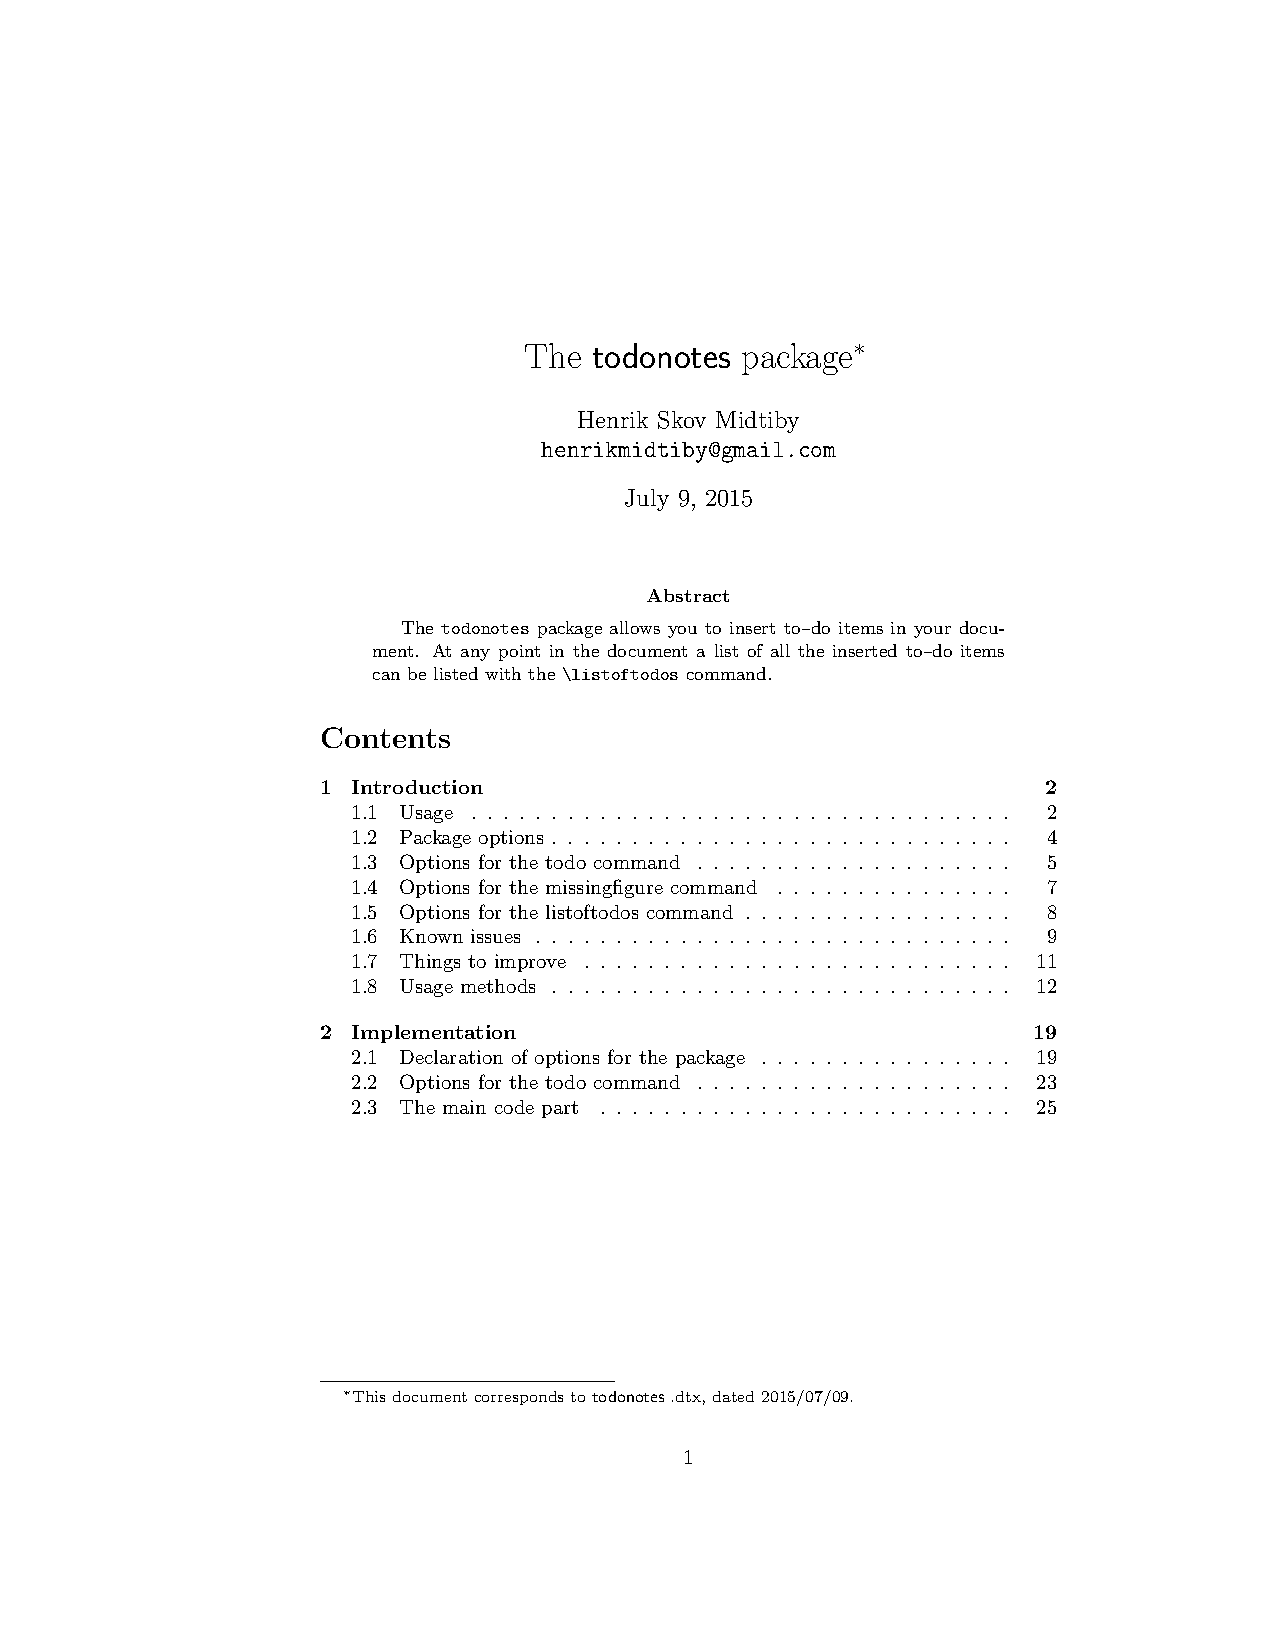
\includepdf[pages=1-3,scale=0.8,frame=true,pagecommand={}]{anexos/todonotes.pdf}

% ---
% Para incluir sem gerar a quebra de página inicial no anexo
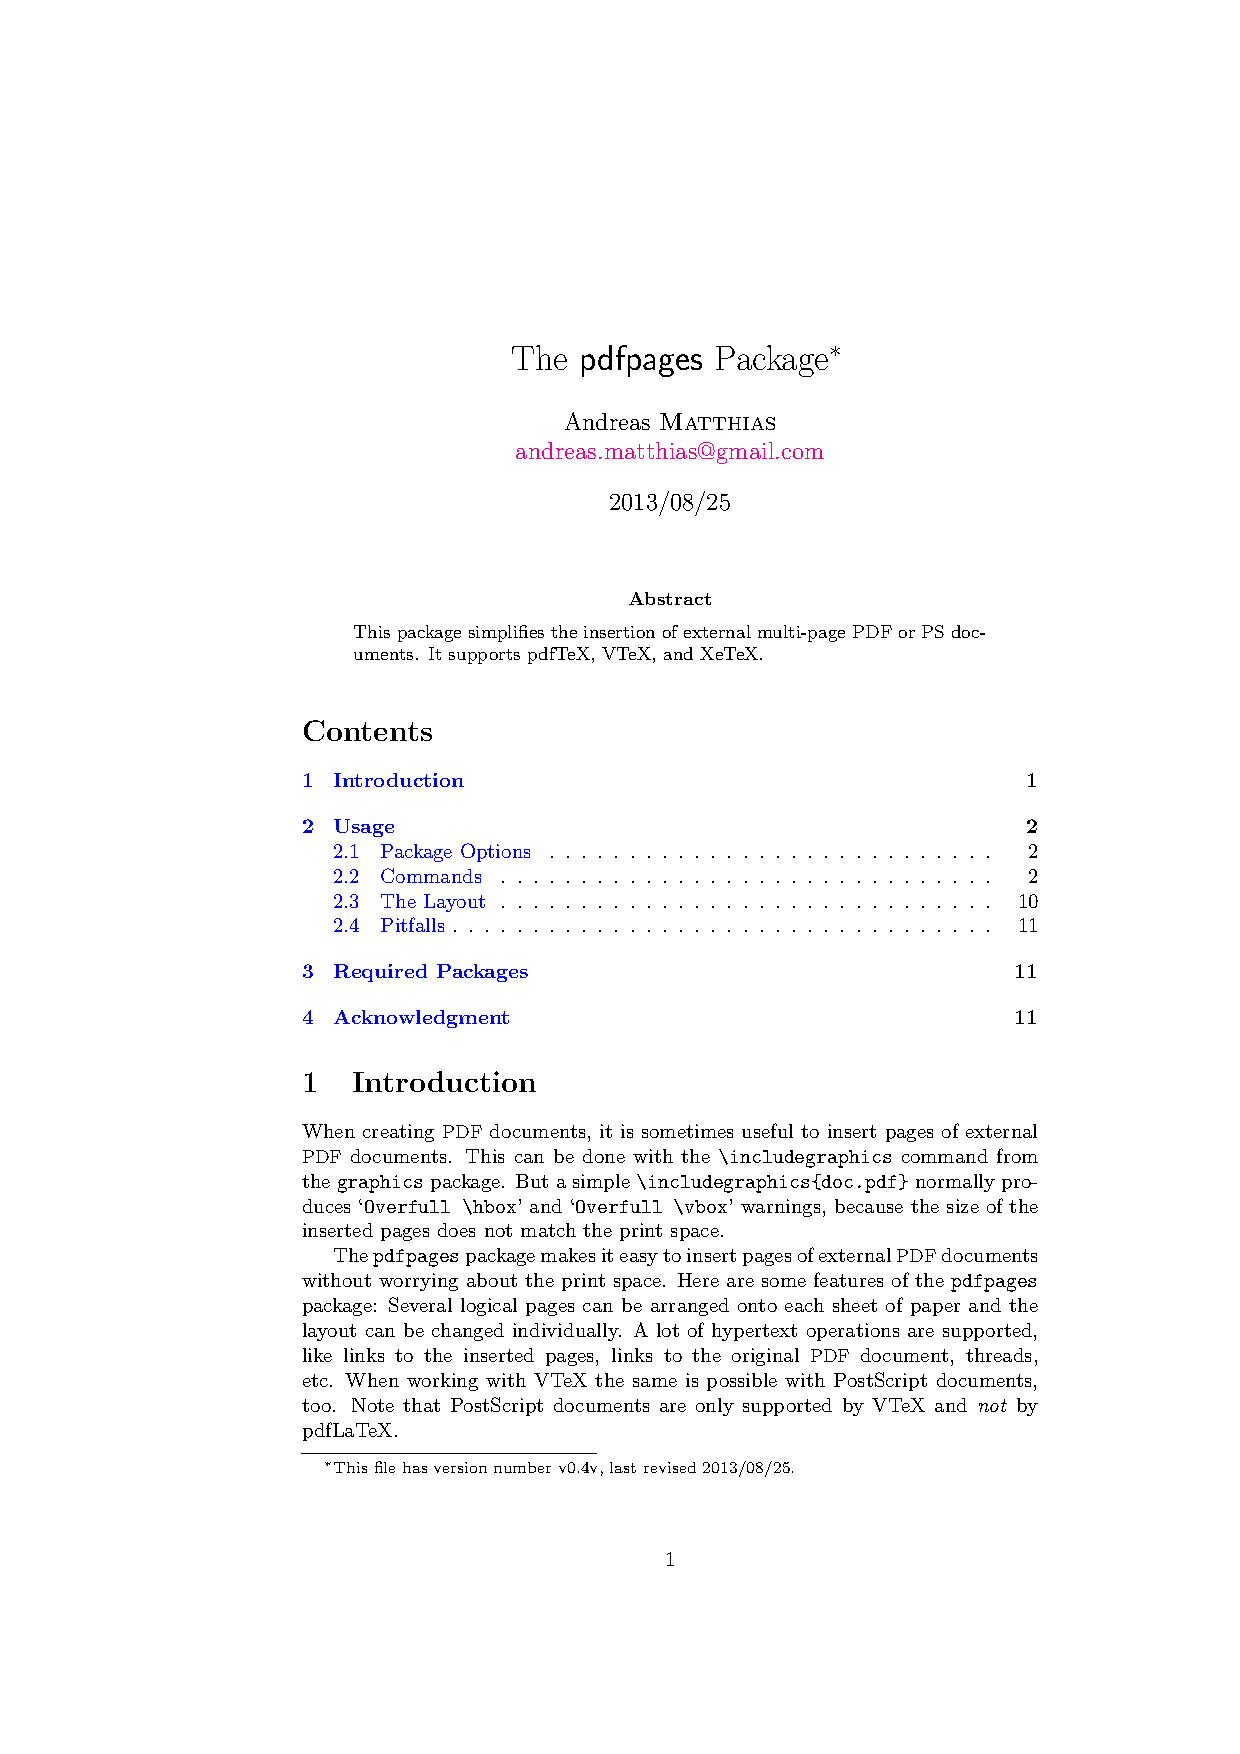
\includepdf[pages=1,scale=0.7,frame=true,pagecommand=\chapter{Manual pdfpages(parcial)}\label{manual-pdfpages}]{anexos/pdfpages.pdf}
\includepdf[pages=2-3,scale=0.8,frame=true,pagecommand={}]{anexos/pdfpages.pdf}

% ---
\chapter{Manual acronym(parcial)}
\index{pdf}
% somente algumas páginas para exemplo sem borda
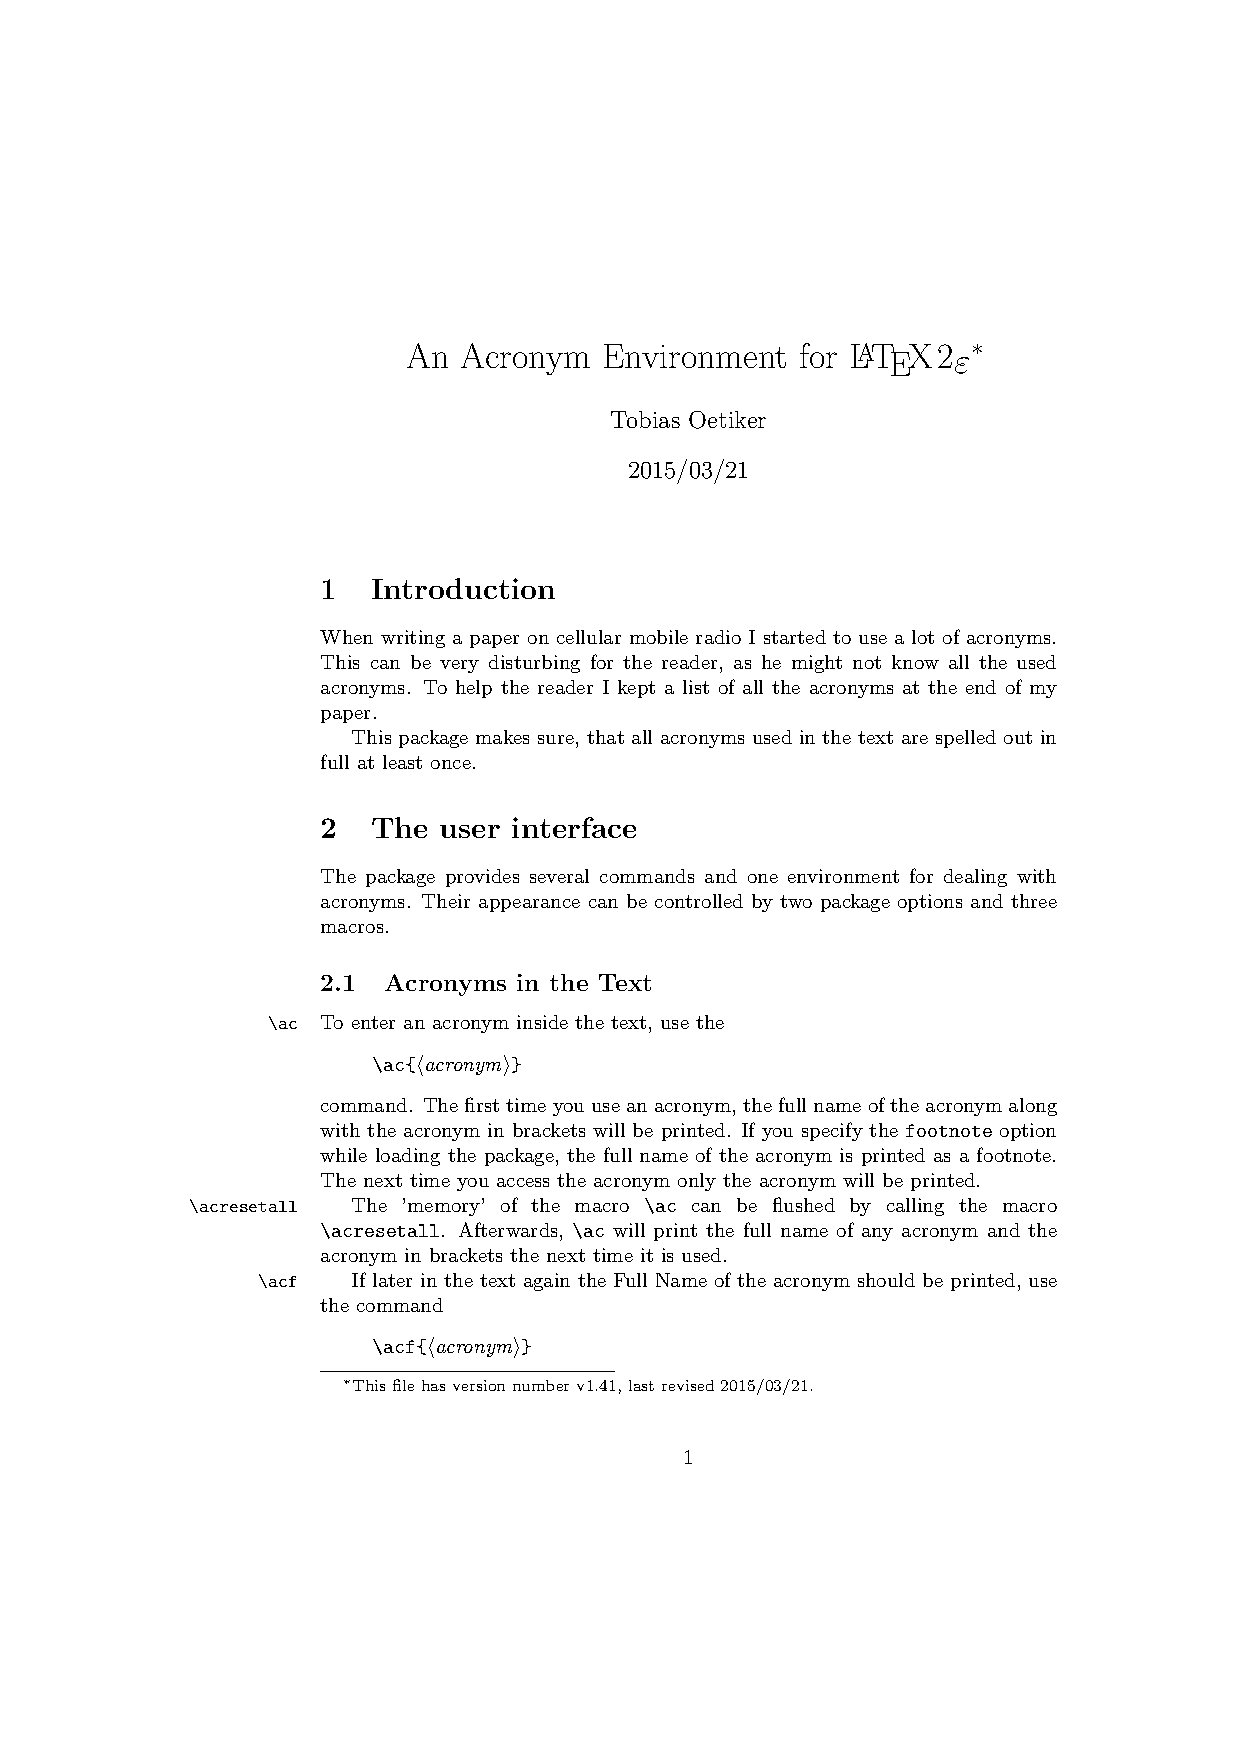
\includepdf[pages=1-3,frame=false,pagecommand={}]{anexos/acronym.pdf}



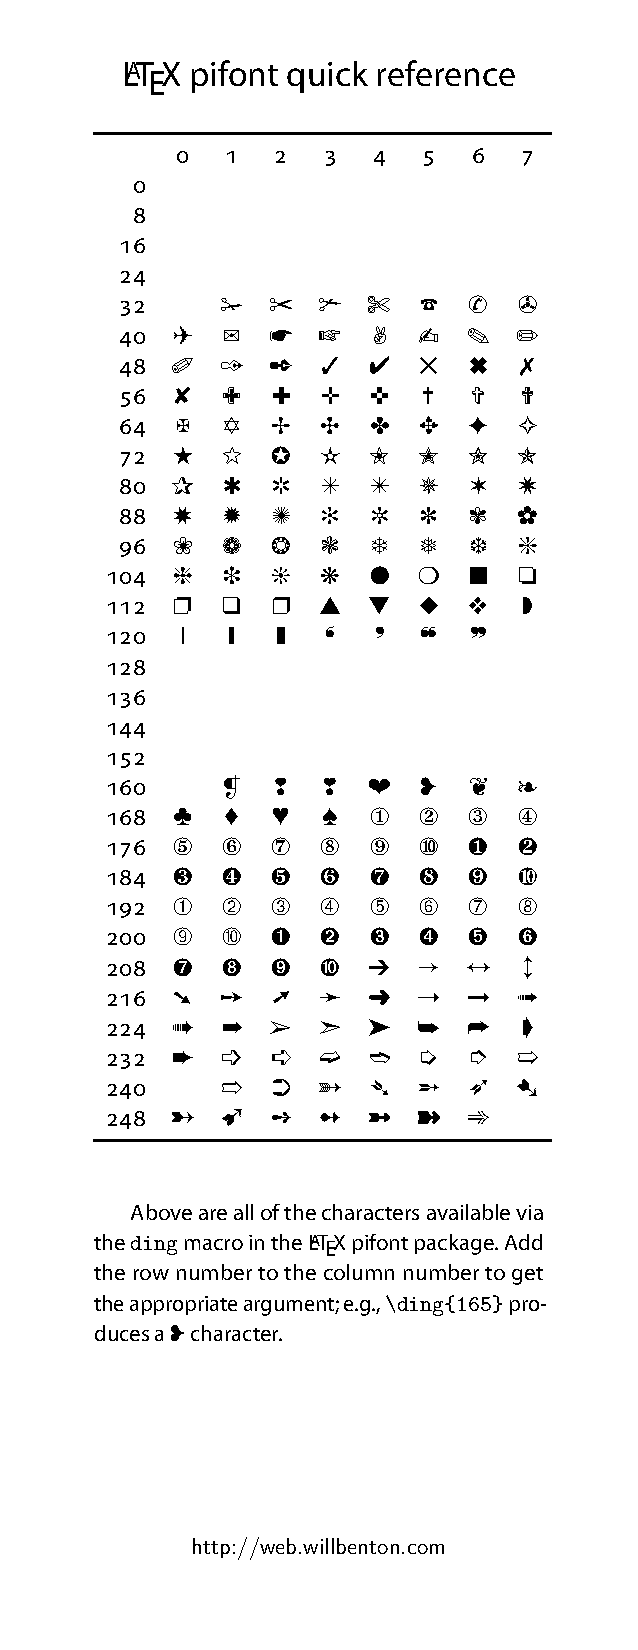
\includepdf[frame=true,scale=0.7,pagecommand=\chapter{Referência Rápida pifont}\label{pifont-quickref}]{anexos/pifont.pdf}


\end{anexosenv}



%---------------------------------------------------------------------
% INDICE REMISSIVO - Quando necessário 
% As palavras indexadas devem ser definidas com \index{} no texto
%---------------------------------------------------------------------
\phantompart
\printindex
\todonum[inline]{remover indice remissivo se não for necessário}

%---------------------------------------------------------------------

\end{document}